\documentclass{beamer}
% personal data
\date{\today}


% language
\usepackage{polyglossia}
\setmainlanguage{english}
\setotherlanguages{german}
\usepackage{microtype}
\usepackage{dcolumn}

\usepackage[style=numeric,
			natbib=true,
			backend=biber]{biblatex}		%Bibliographie
\usepackage[autostyle=true,
			 german=quotes]
			 {csquotes}					%Anführungszeichen
\usepackage{blindtext}


%math and theorems
\usepackage{amsmath}
\usepackage{amssymb}
\usepackage{amsopn}					%Matheoperatoren
\usepackage[amsmath,thmmarks,hyperref]{ntheorem}
\usepackage{mathtools}
\usepackage{mathdots}					%Punkte
\usepackage{dsfont}
\usepackage{upgreek}					%Griechische Buchstaben
\usepackage{bbm}						%Mengensymbol
\usepackage{physics}					%Physiksymbole
\usepackage{relsize}						%Größenangaben
\usepackage[separate-uncertainty,
			per-mode=symbol]
			{siunitx}					%Einheiten
%\usepackage{tikz}						%Zeichnen
\usepackage{upgreek}					%Griechische Buchstaben
\usepackage{enumitem}
\setlist{nolistsep}


%useful packages
%\usepackage{geometry}
\usepackage{xcolor}
\usepackage{graphicx}
\usepackage{float}
\usepackage{csquotes}
\usepackage{todonotes}
\usepackage{booktabs}
\usepackage{array}
\usepackage[labelfont=bf]{caption}
\usepackage{wrapfig}
\usepackage{enumitem}
%\usepackage{xr} % cross referencing
%\usepackage{titling}
%\usepackage{titlesec}
%\usepackage[Bjornstrup]
%			{fncychap}					%Kapitellayout


\setmainfont{Linux Libertine O}
\setsansfont{Linux Biolinum O}

\usepackage{scrhack}					%Verbesserung Pakete
\usepackage{xltxtra}						%fontec


\newcommand{\im}{\mathrm{i}}
\newcommand{\e}{\mathrm{e}}
\renewcommand{\pi}{\uppi}
\renewcommand{\epsilon}{\varepsilon}


\addbibresource{bibliography.bib}

%color settings
\definecolor{myred}{RGB}{196,19,47} 
\definecolor{myblue}{RGB}{0,139,139}


%appendix
\usepackage[toc,page]{appendix}

%killing indent
\setlength{\parindent}{0pt}
\usepackage{multicol}
\usepackage{siunitx}
\usepackage{hyperref}


\title{Atmosphärische Spurensuche}
\author{Aaron Mielke \& Thomas Ackermann}
\date{\today}

\begin{document}

\maketitle

% \tableofcontents

\begin{frame}
\frametitle{Einführung}
    \section{Einführung}
    Wichtig in diesem Versuch: Tropos- und Stratosphäre\\
    Beschränkung auf die Spurengase \ch{O3}, \ch{O4} und \ch{NO2} 
    \begin{figure}[h]
        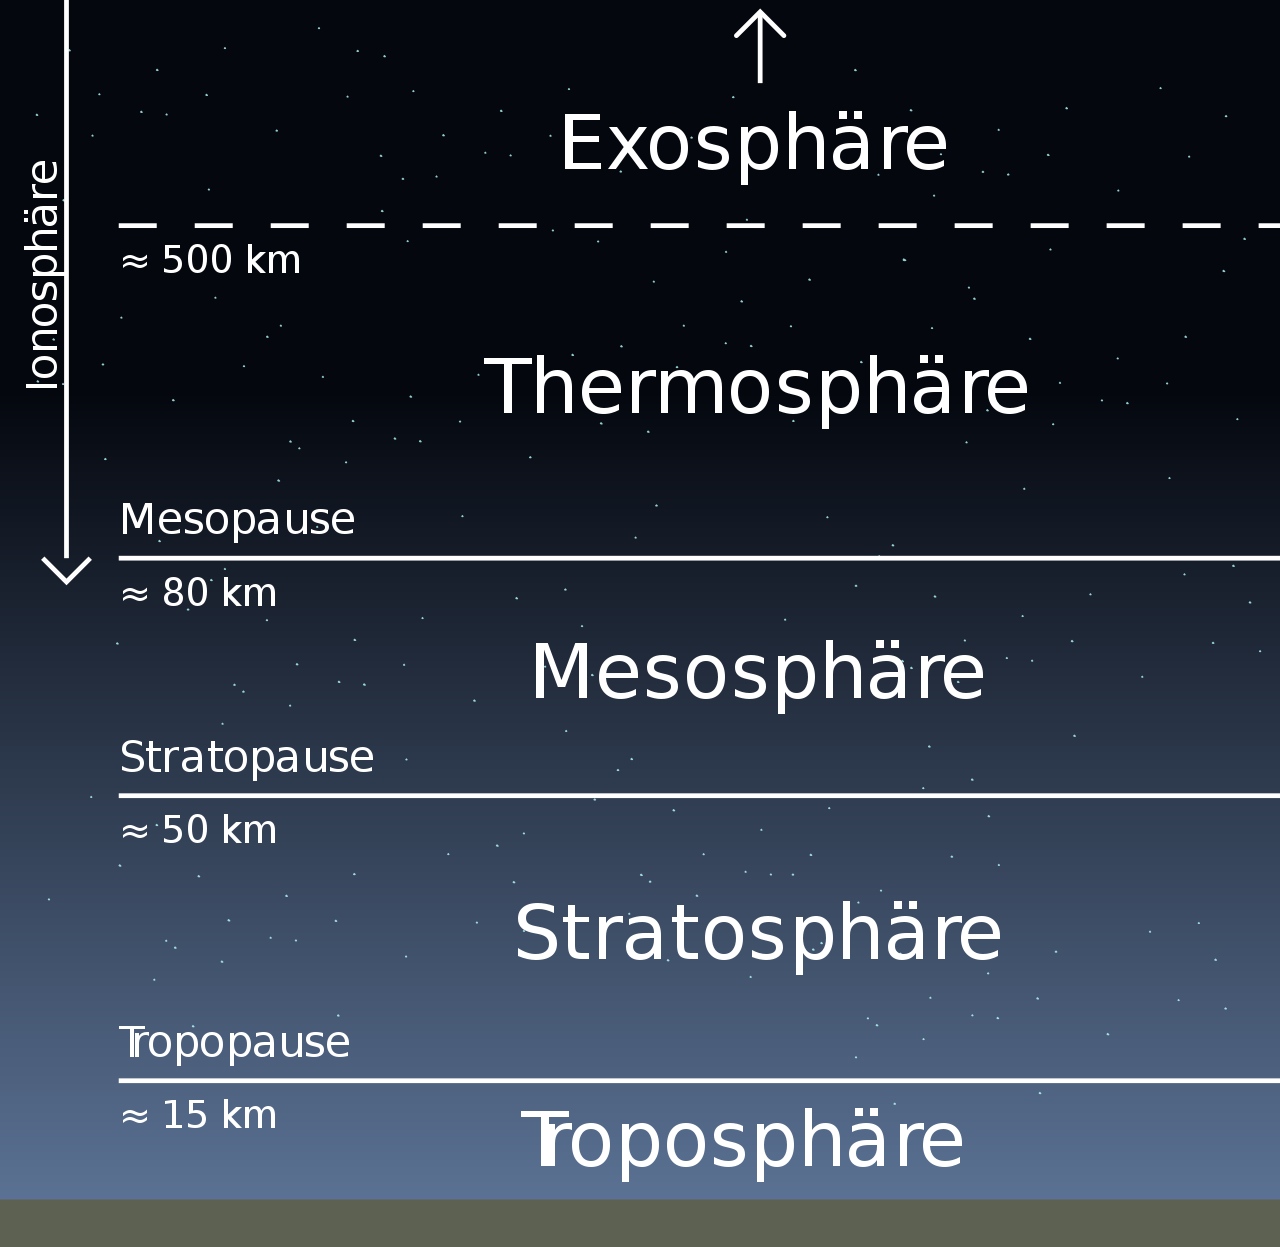
\includegraphics[width=0.4\textwidth]{fig/photo/erdatmosphäre.png}
    \end{figure}
\end{frame}


\begin{frame}
    \frametitle{Inhaltsangabe}
    \begin{itemize}
        \item[-] Theoretische Grundlagen
    \vfill
\item[-] Labormessungen
    \vfill
\item[-] Atmosphärische Messungen 
\end{itemize}
\end{frame}


% \begin{frame}
% \frametitle{Messgrößen}
%     \begin{itemize}
%         \item Konzentration: Moleküle pro Volumeneinheit
%         \item Mischverhältnis: Relativer Anteil von Spurengas zu Luftmenge
%         \item Column density: $CD = \int \rho (s) \dd s$
%     \end{itemize}
% \end{frame}

\begin{frame}
    \frametitle{DOAS}
    \section{Theoretische Grundlagen}
    \begin{columns}
    \column{.6\textwidth}
    \begin{itemize}
        \item[-] Verwendung: Konzentration von Spurengasen bestimmen
        \item[-] Benutze Chrakteristische Profile von Molekülen
        \item[-] Vergleich von optischen Dichten
        \item[-] Bestimmung Konzentration in Tropo- oder Stratosphäre
    \end{itemize}
    \column{0.4\textwidth}
    \begin{minipage}{80mm}
        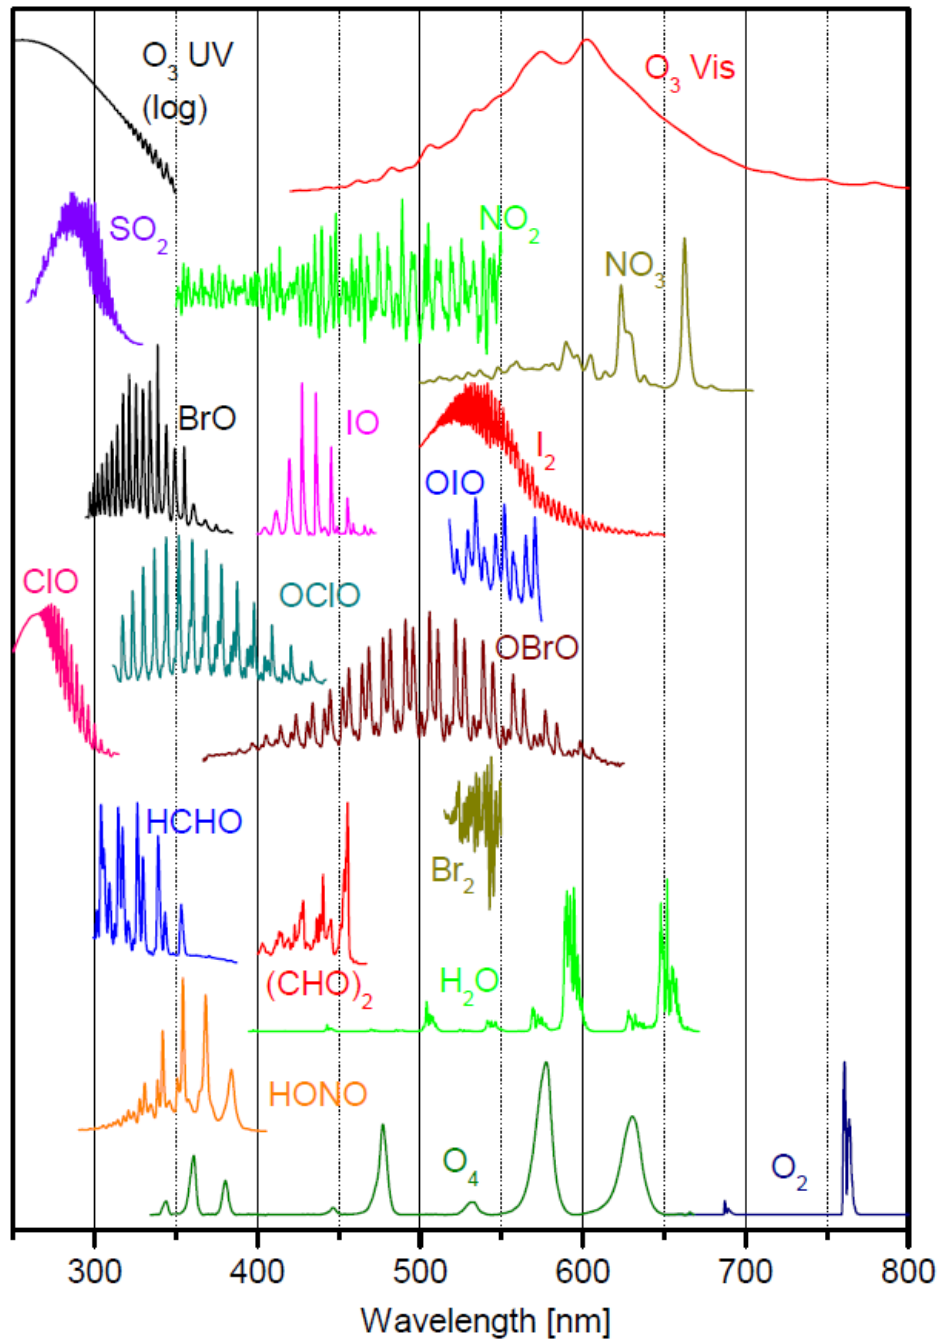
\includegraphics[width=0.5\textwidth]{fig/gas_spectra.png}
    \end{minipage}
    \end{columns}
\end{frame}

\begin{frame}
    \frametitle{Lambert-Beer}
    \begin{figure}[h]
        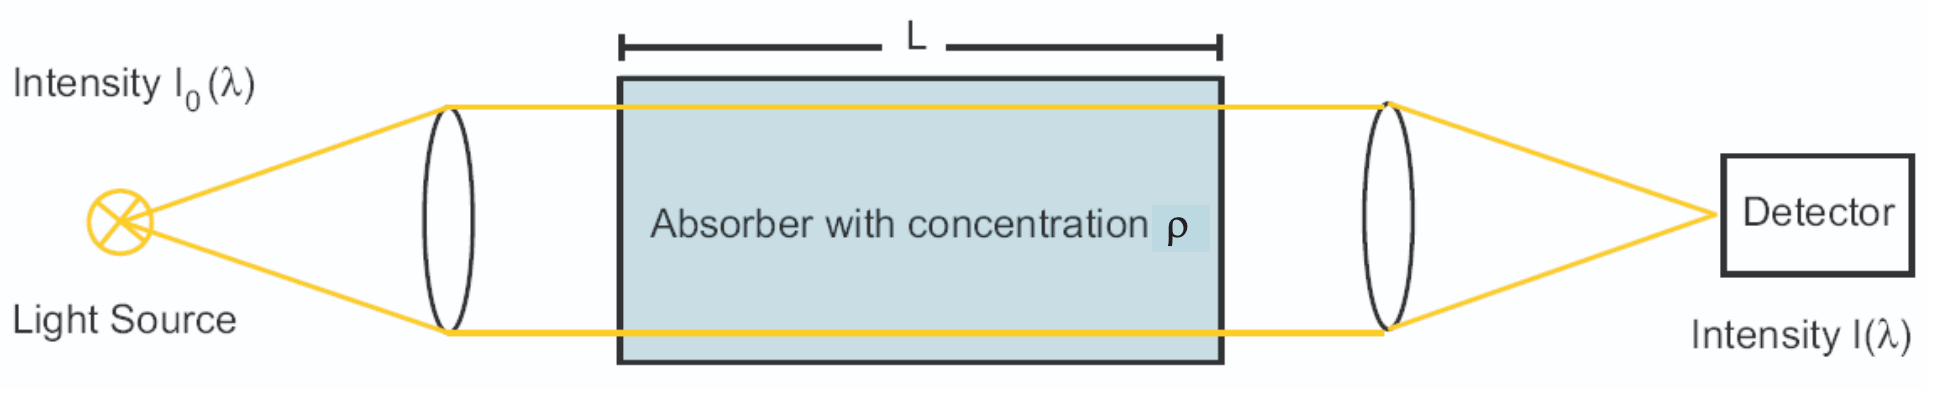
\includegraphics[width=0.6\textwidth]{fig/lambert_beer.png}
    \end{figure}
    \begin{align}
    I(\lambda, L) = I_0 (\lambda) \exp (- \rho  L \sigma (\lambda) )
    \end{align}
    \begin{itemize}
        \item $L$ Länge des Mediums
        \item $\rho$ Dichte
        \item $\sigma (\lambda)$ Absorptionswirkungsquerschnitt % Absorptionswirkungsquerschnitt ist wahrscheinlichkeit dass bei bestimmen winkel absorption stattfindet
    \end{itemize}
\end{frame}


\begin{frame}
    \frametitle{DOAS-Fit}
    Forme Lambert-Beer um:
\begin{align}
    \tau = \log \frac{I}{I_0} = - \rho L \sigma (\lambda).
\end{align}
$\tau$ : Optische Dichte\\
Erstelle Fit durch Minimierung von
    \begin{align}
        \chi^2 = ( \log \frac{I_0}{I} - \rho L \sigma )^2. 
    \end{align}
\end{frame}


\begin{frame}
    \frametitle{Kurzband Effekte}
Fraunhofer Referenzspektrum
    \begin{itemize}
        \item Berücksichtigung der Strukturen der Sonne
    \end{itemize}
    \begin{figure}[h]
        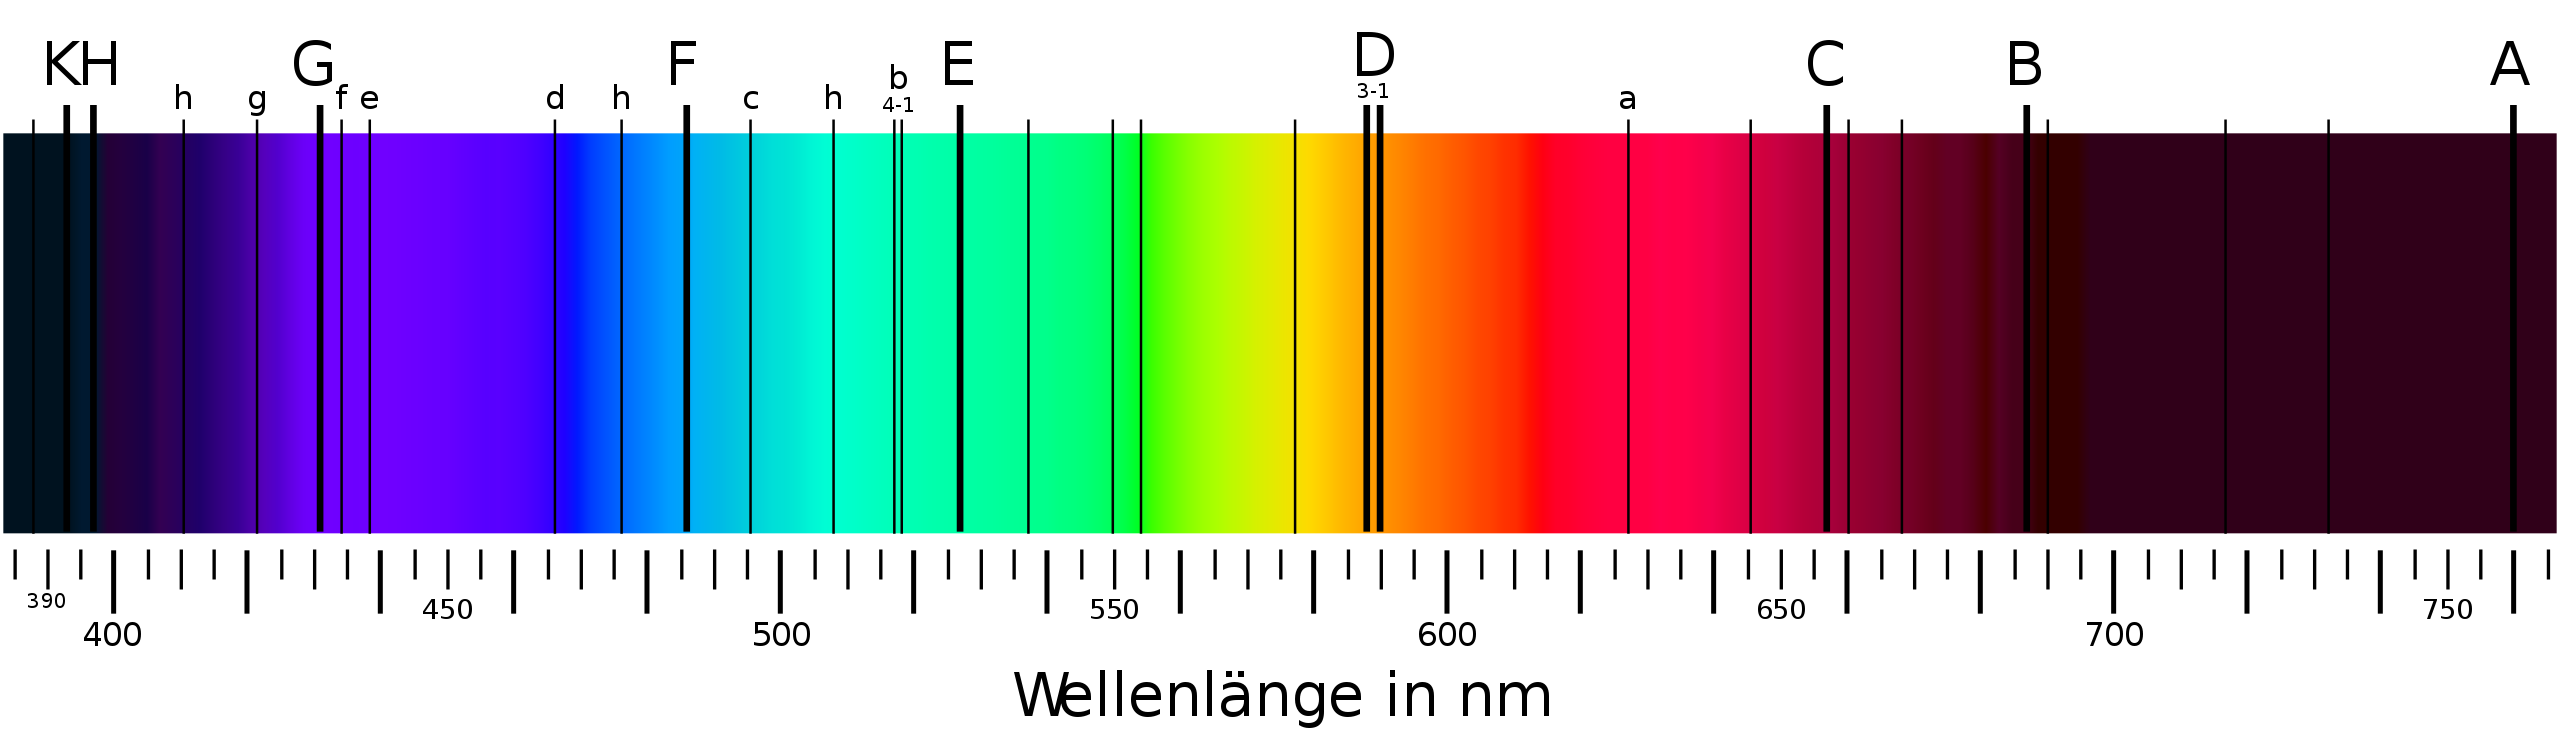
\includegraphics[width=0.7\textwidth]{fig/fraunhofer_linien.png}
    \end{figure}
\end{frame}

\begin{frame}
\frametitle{Kurzband Effekte}
    Ring-Effekt
    \begin{itemize}
        \item Inelastische Raman-Streuung
        \item Wellenlängen ändern sich
    \end{itemize}
\end{frame}

\begin{frame}
    \frametitle{Breitband Effekte}
    \begin{itemize}
        \item Elastische Streuung von Sonnenlicht 
        \item $\to$ Mie und Reyleigh Streuung
        \item Summe aus Streuung und Absorbtion : \textit{Extinktion} $\epsilon_M$ und $\epsilon_R$
    Rayleigh: $\sim \lambda^{-4}$\\
    Mie: keine starke $\lambda$ Abhängigkeit
    \end{itemize}
\end{frame}

\begin{frame}
    \frametitle{Breitband Effekte}
    \begin{figure}
    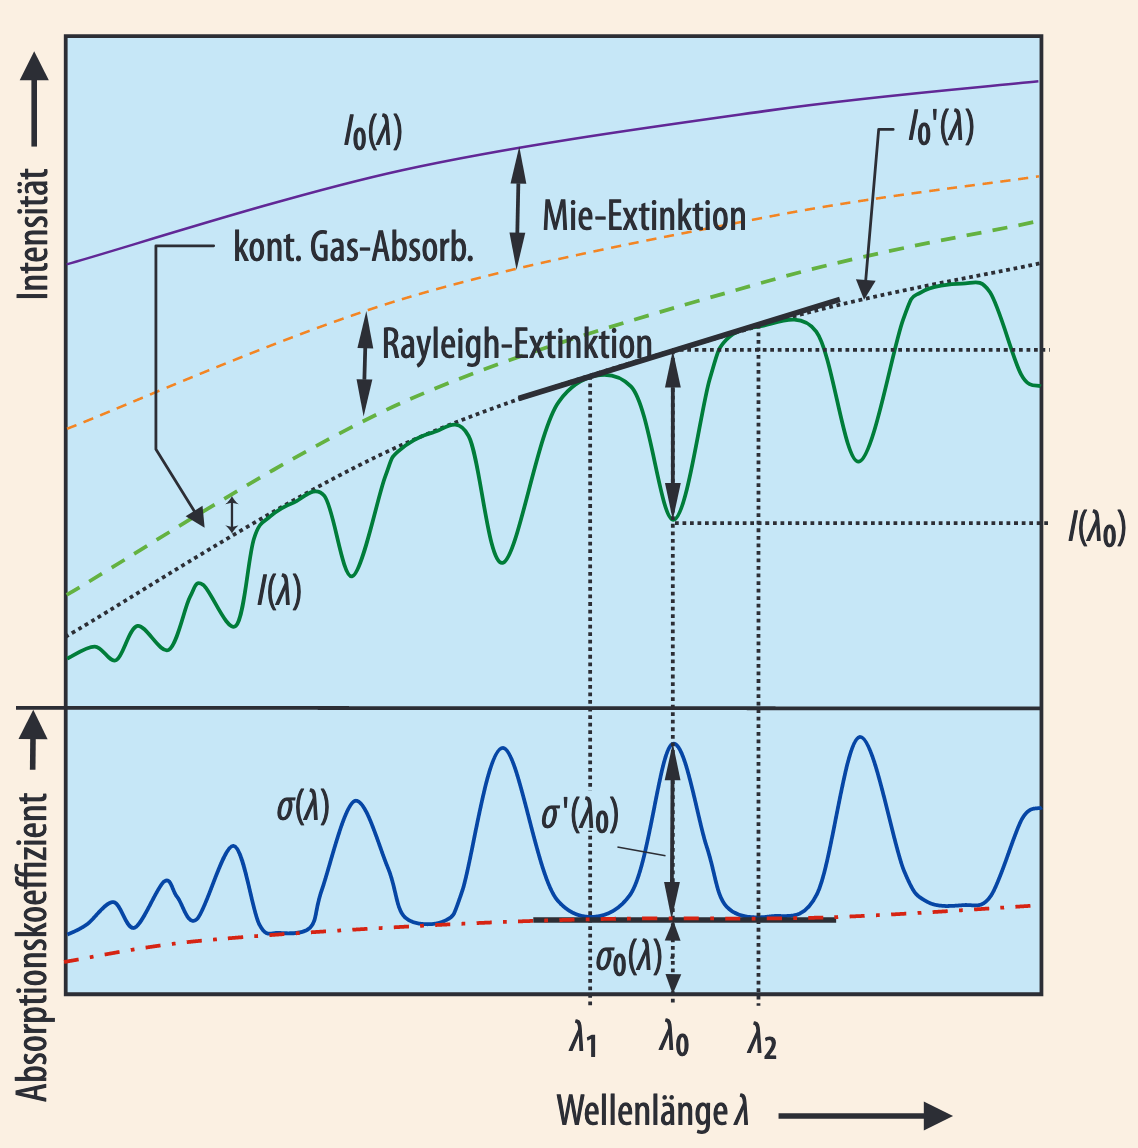
\includegraphics[width=0.7\linewidth]{fig/rayleigh_mie.png}
    \end{figure}
\end{frame}


\begin{frame}
    \frametitle{Modifiziertes Lamber-Beer Gesetz}
    \begin{align}
        I = I_0 \exp(-R - \sum_i \sigma_i S_i) \exp\left(-L (\sigma_{i0}\rho_0) + \epsilon_R + \epsilon_M\right)
    \end{align}
    Erste Exponentialfunktion: Kurzband Effekte\\
    Zweite Exponentialfunktion: Breitband Effekte\\
    \pause
    Neues $\chi^2$
    \begin{align}
        \chi^2 = \left( \log\frac{I_0 + I_\text{Ofs}}{I} - R - \sum_i \sigma_i S_i - \sum_k b_k \lambda^k \right)^2.
    \end{align}
\end{frame}

\begin{frame}
    \frametitle{Versuchsaufbau}
    \section{Versuchsaufbau}
    Was sollte hier nochmal hin?
    Bild von Spektrometer
\end{frame}

\begin{frame}
    \section{Auflösungs des Spektrometers}
    \frametitle{Auflösung des Spektrometers}
    \begin{figure}[h]
        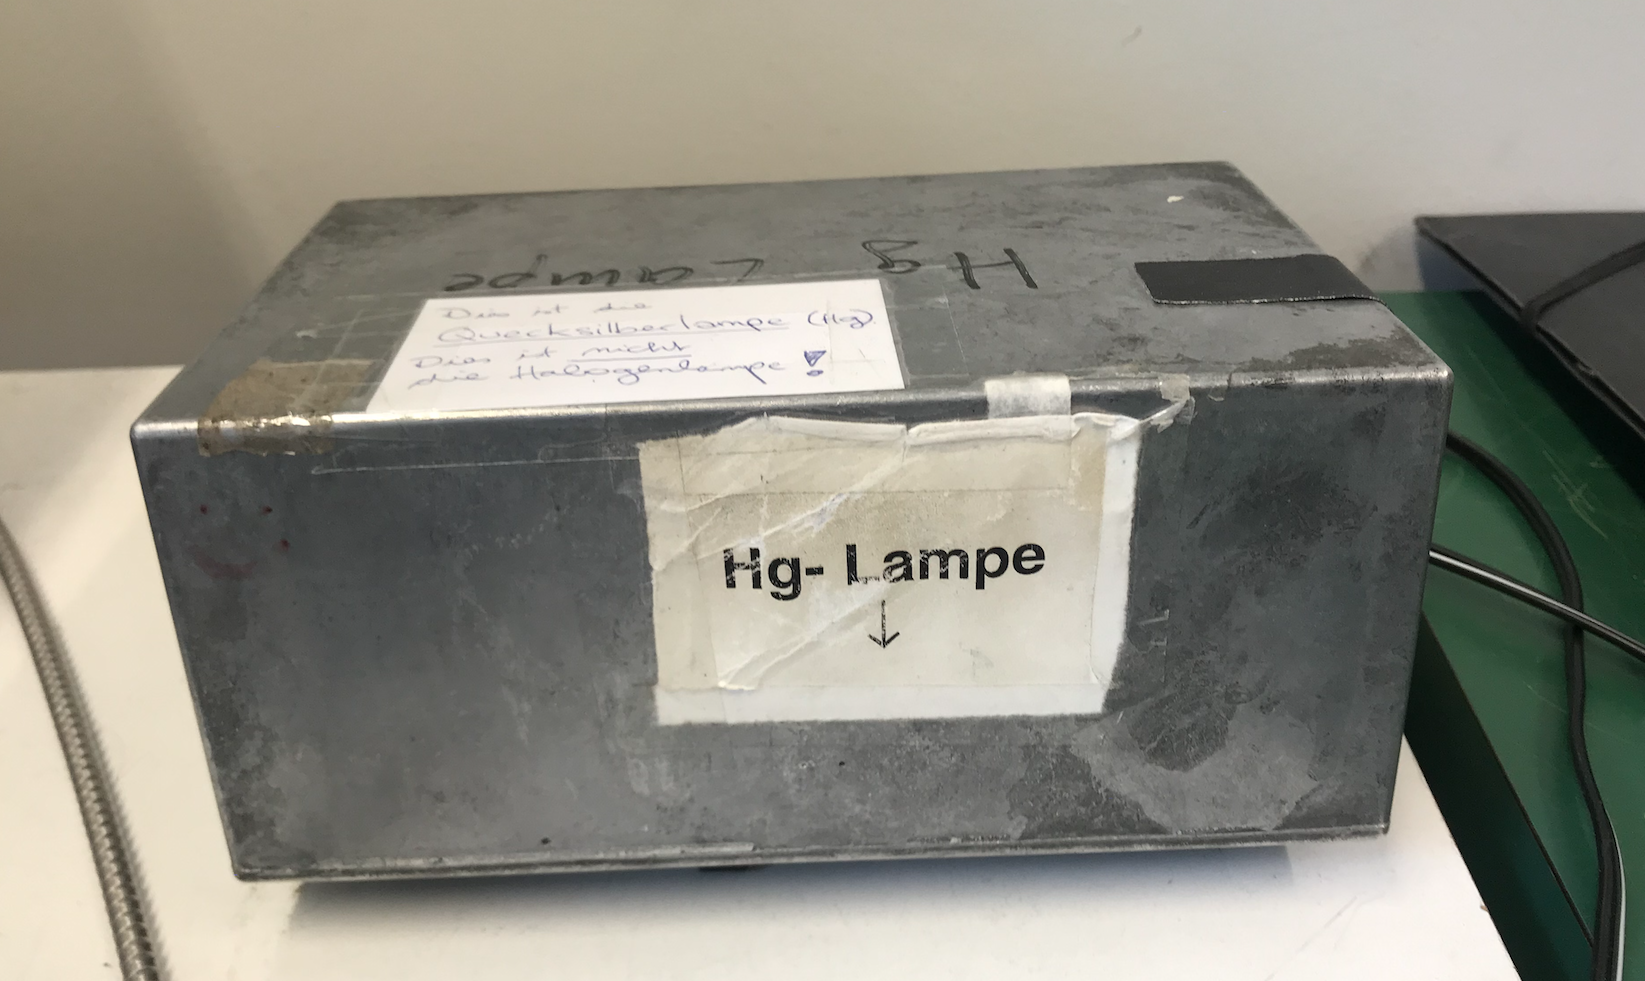
\includegraphics[width=0.5\textwidth]{fig/photo/hg_lampe.png}
    \end{figure}
\end{frame}

\begin{frame}
    \framtitle{Spektrum der Quecksilberlampe}

    \begin{figure}[h]
        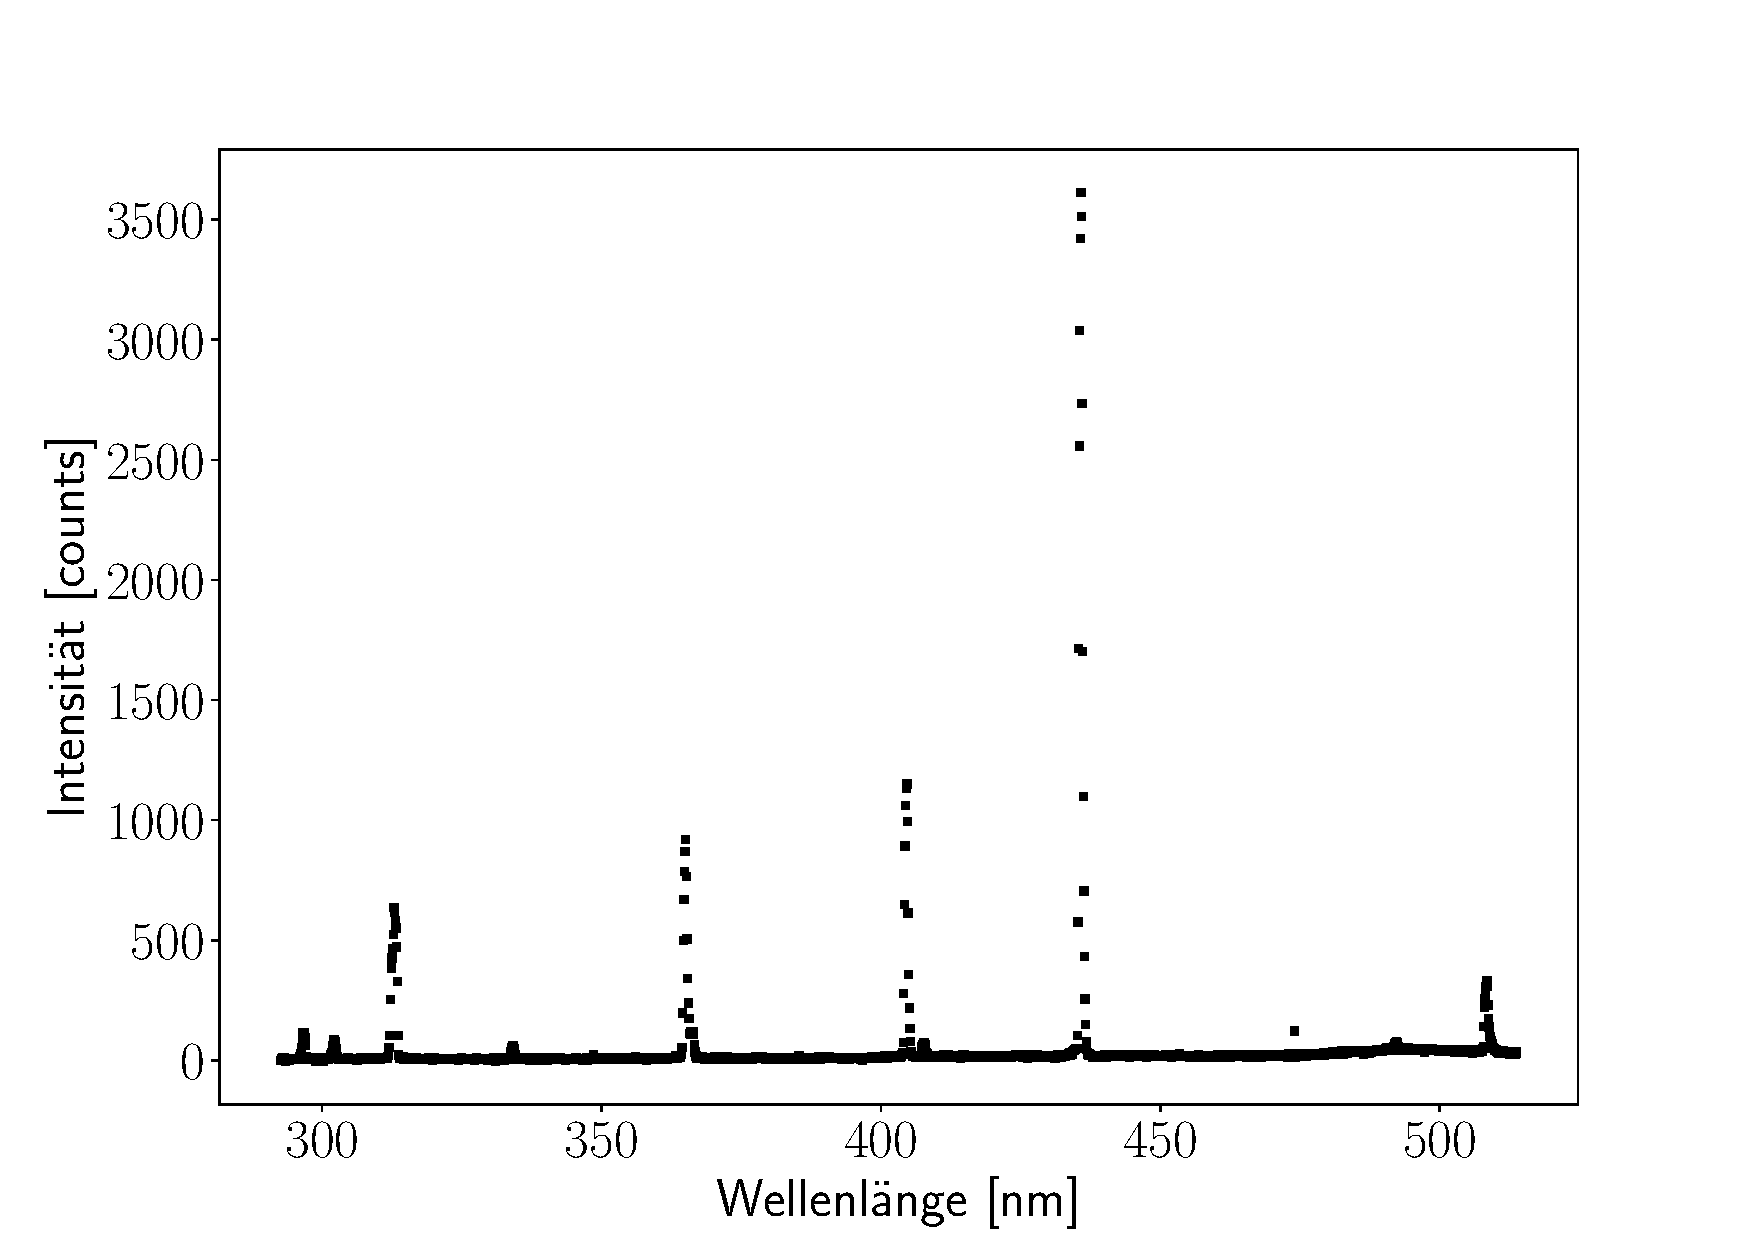
\includegraphics[width=\textwidth]{fig/hg_spectrum.pdf}
    \end{figure}
\end{frame}
\begin{frame}
    \frametitle{Auflösung des Spektrometers} 
    \begin{tabular*}{\linewidth}{@{\extracolsep{\fill}} c c c}
    \toprule
    Maximum & Wellenlänge & FWHM [\si{nm}] \\
    \midrule
    1 & $\sim 313$ & $1.2 \pm 0.1$ \\
    2 & $\sim 365$ & $0.8 \pm 0.1$ \\
    3 & $\sim 404$ & $0.6 \pm 0.1$ \\
    4 & $\sim 436$ & $0.7 \pm 0.1$ \\
    \bottomrule
\end{tabular*}
\end{frame}

\begin{frame}
    \section{Labormessungen}
    \frametitle{Halogenlampen Messung}

    \begin{figure}[h]
        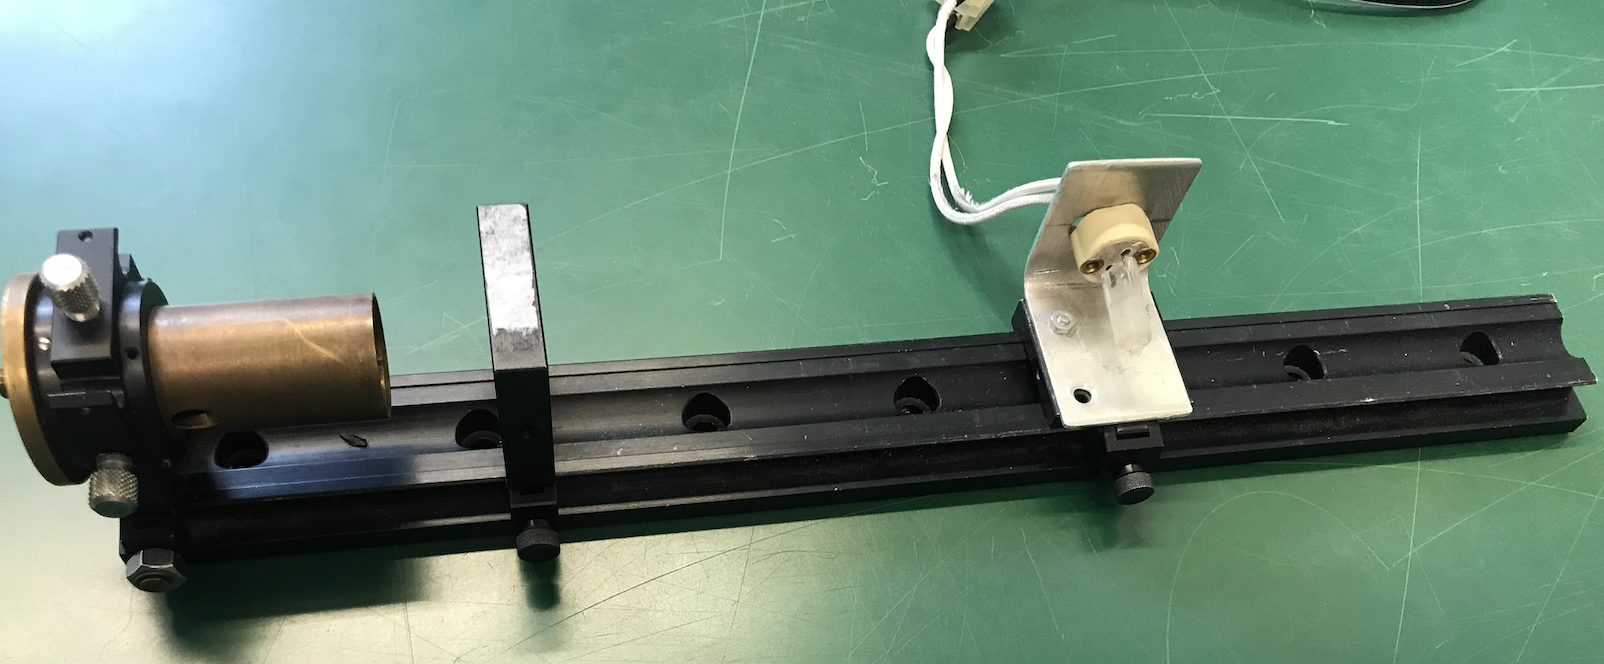
\includegraphics[width=0.7\textwidth]{fig/photo/aufbau_1.png}
    \end{figure}

    \begin{figure}[h]
        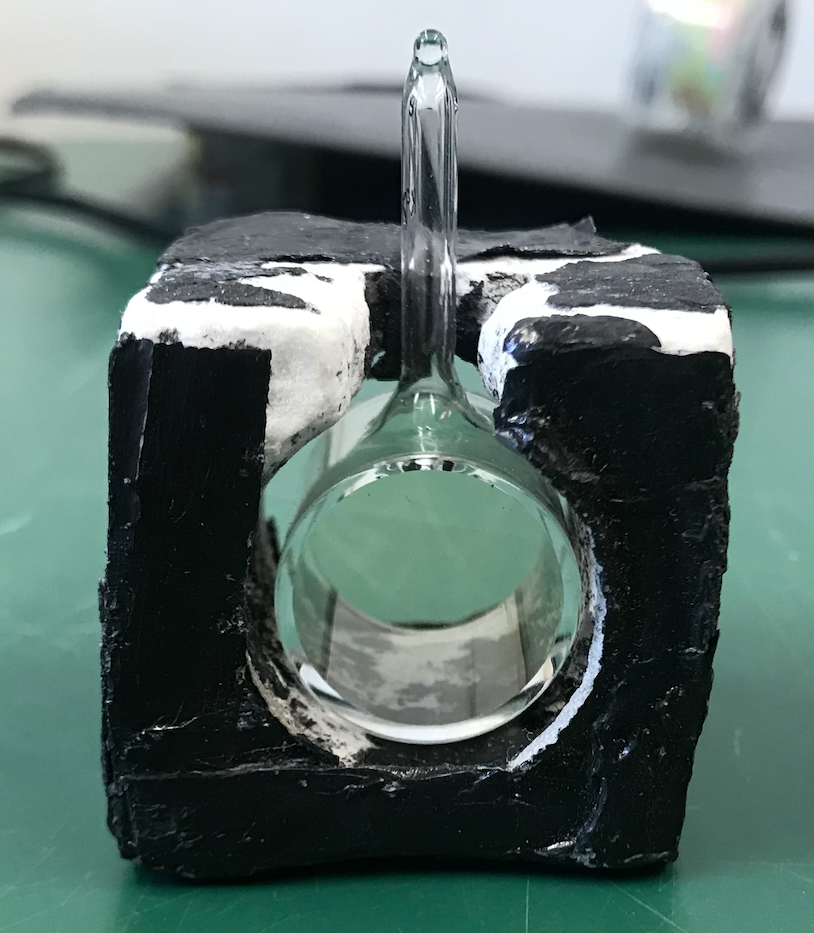
\includegraphics[width=0.3\textwidth]{fig/photo/glas_test.png}
    \end{figure}
\end{frame}

\begin{frame}
    \frametitle{Halogenlampen Messung}
\begin{itemize}
    \item Atmosphärische Einflüsse vernachlässigbar
\end{itemize}
\begin{align}
 \to \tau = \sigma_{\ch{NO2}}(\lambda) \cdot \rho_{\ch{NO2}} \cdot L
\end{align}
    \begin{itemize}
    \item Fitbereich: Suche nach Überlagerung mit \ch{NO2} Referenz
    \item Hier verwendet: $(413.46 - 477.25) \si{nm}$
    \end{itemize}
    \begin{align}
\to \rho_\ch{NO2} = (2.48 \pm 0.12) \cdot 10^{20} \si{\frac{\text{Moleküle}}{\ell}}
    \end{align}
\end{frame}

\begin{frame}
    \section{Atmosphärische Messungen}
    \frametitle{Versuchsaufbau}
    \begin{figure}[h]
        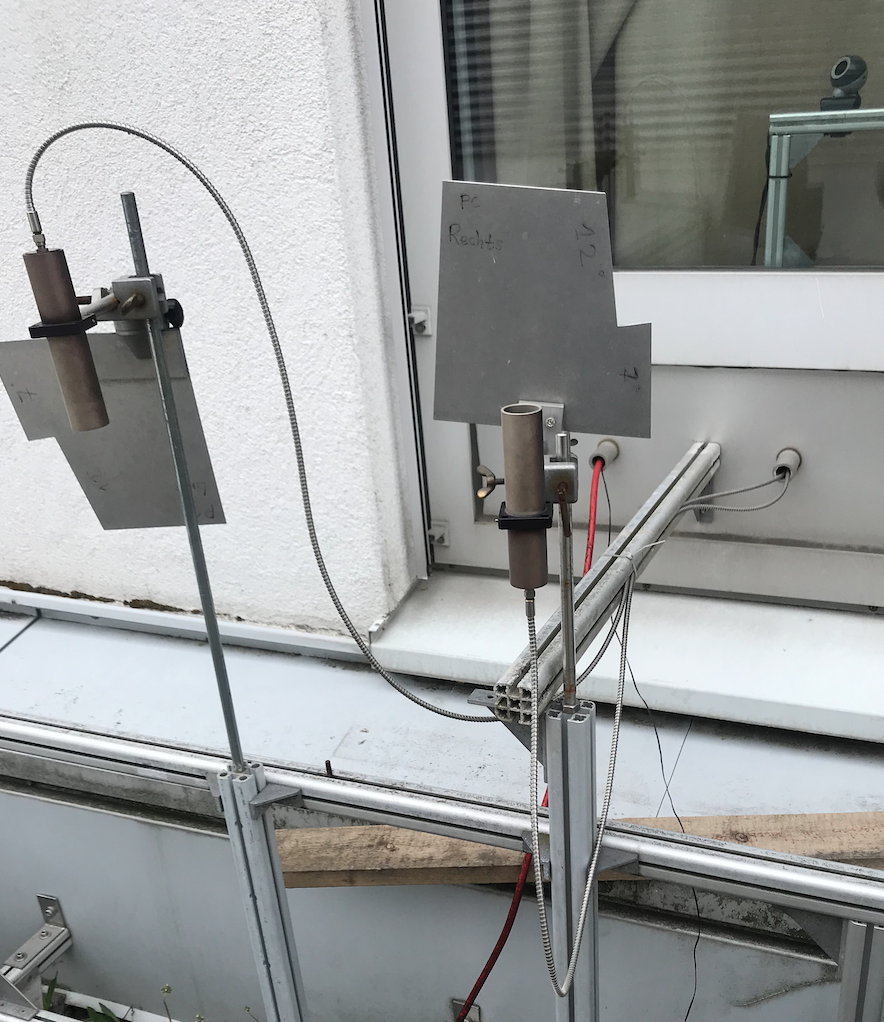
\includegraphics[width=0.5\textwidth]{fig/photo/aufbau_2.png}
    \end{figure}
\end{frame}


\begin{frame}
    \frametitle{Atmosphärische Messungen}
    \begin{itemize}
        \item Jetzt erweitertes Lambert-Beer Gesetz
        \item Untersuchung von SCD
    \end{itemize}
\end{frame}


\begin{frame}
    \frametitle{Tagesmessung \ch{NO2}}
\begin{center}
    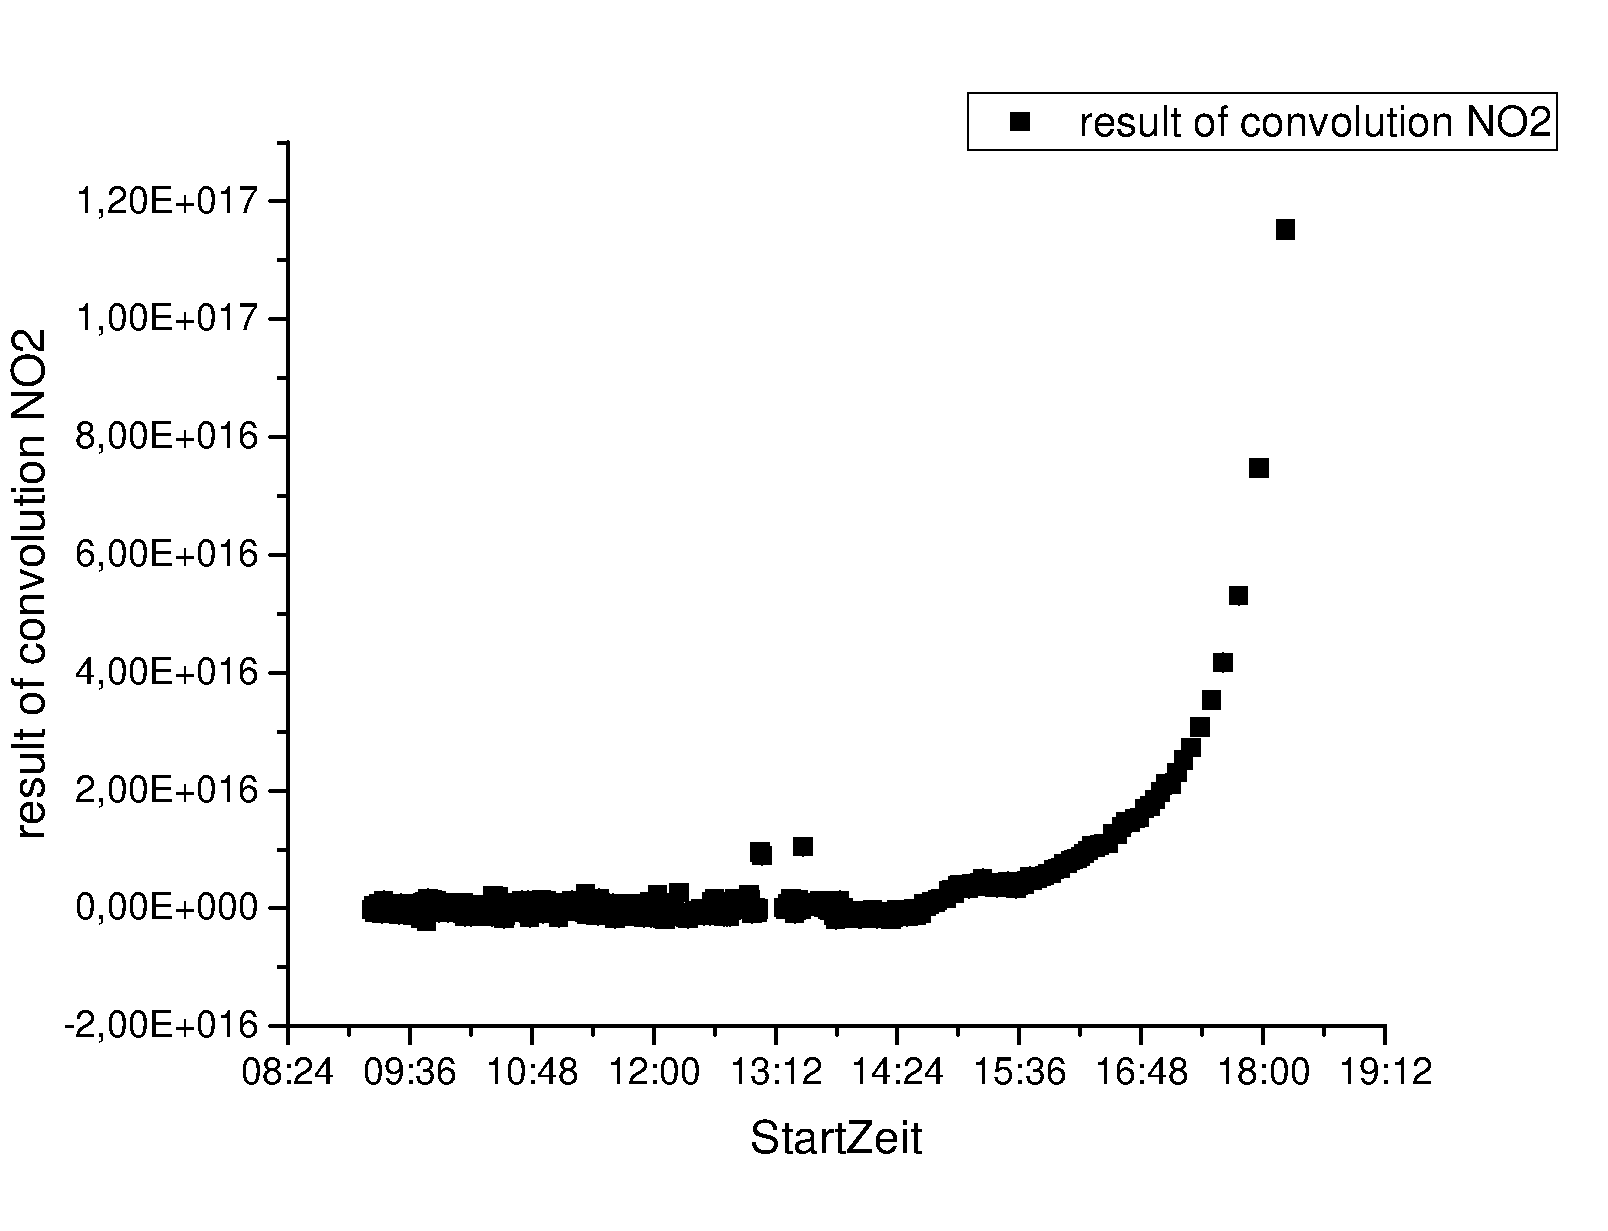
\includegraphics[width=.9\linewidth]{fig/SCD_Time_Plot_NO2.pdf}
    \captionof{figure}{$\Delta \text{SCD}$ von \ch{NO2} über den Tag des 24.04.2019}
    \label{fig:delta_SCD_time_NO2}
\end{center}
\end{frame}

\begin{frame}
    \frametitle{Tagesmessung \ch{NO2}}
    Am Morgen:
    \begin{align}
        \ch{NO2} + h \nu \to \ch{NO} + \ch{O}(^3\text{P})
    \end{align}
    \pause
    Gleichzeitig Dissoziation:
    \begin{align}
        \ch{N2O5} + h \nu \to \ch{NO2} + \ch{NO3}
    \end{align}
    \pause
    Reagiert weiter:
    \begin{align}
        \ch{NO3} + h \nu \to \ch{NO} + \ch{O2}\\
        \ch{NO3} + h \nu \to \ch{NO2} + \ch{O}
    \end{align}
\end{frame}

\begin{frame}
    \frametitle{Tagesmessung \ch{O3}}
\begin{center}
    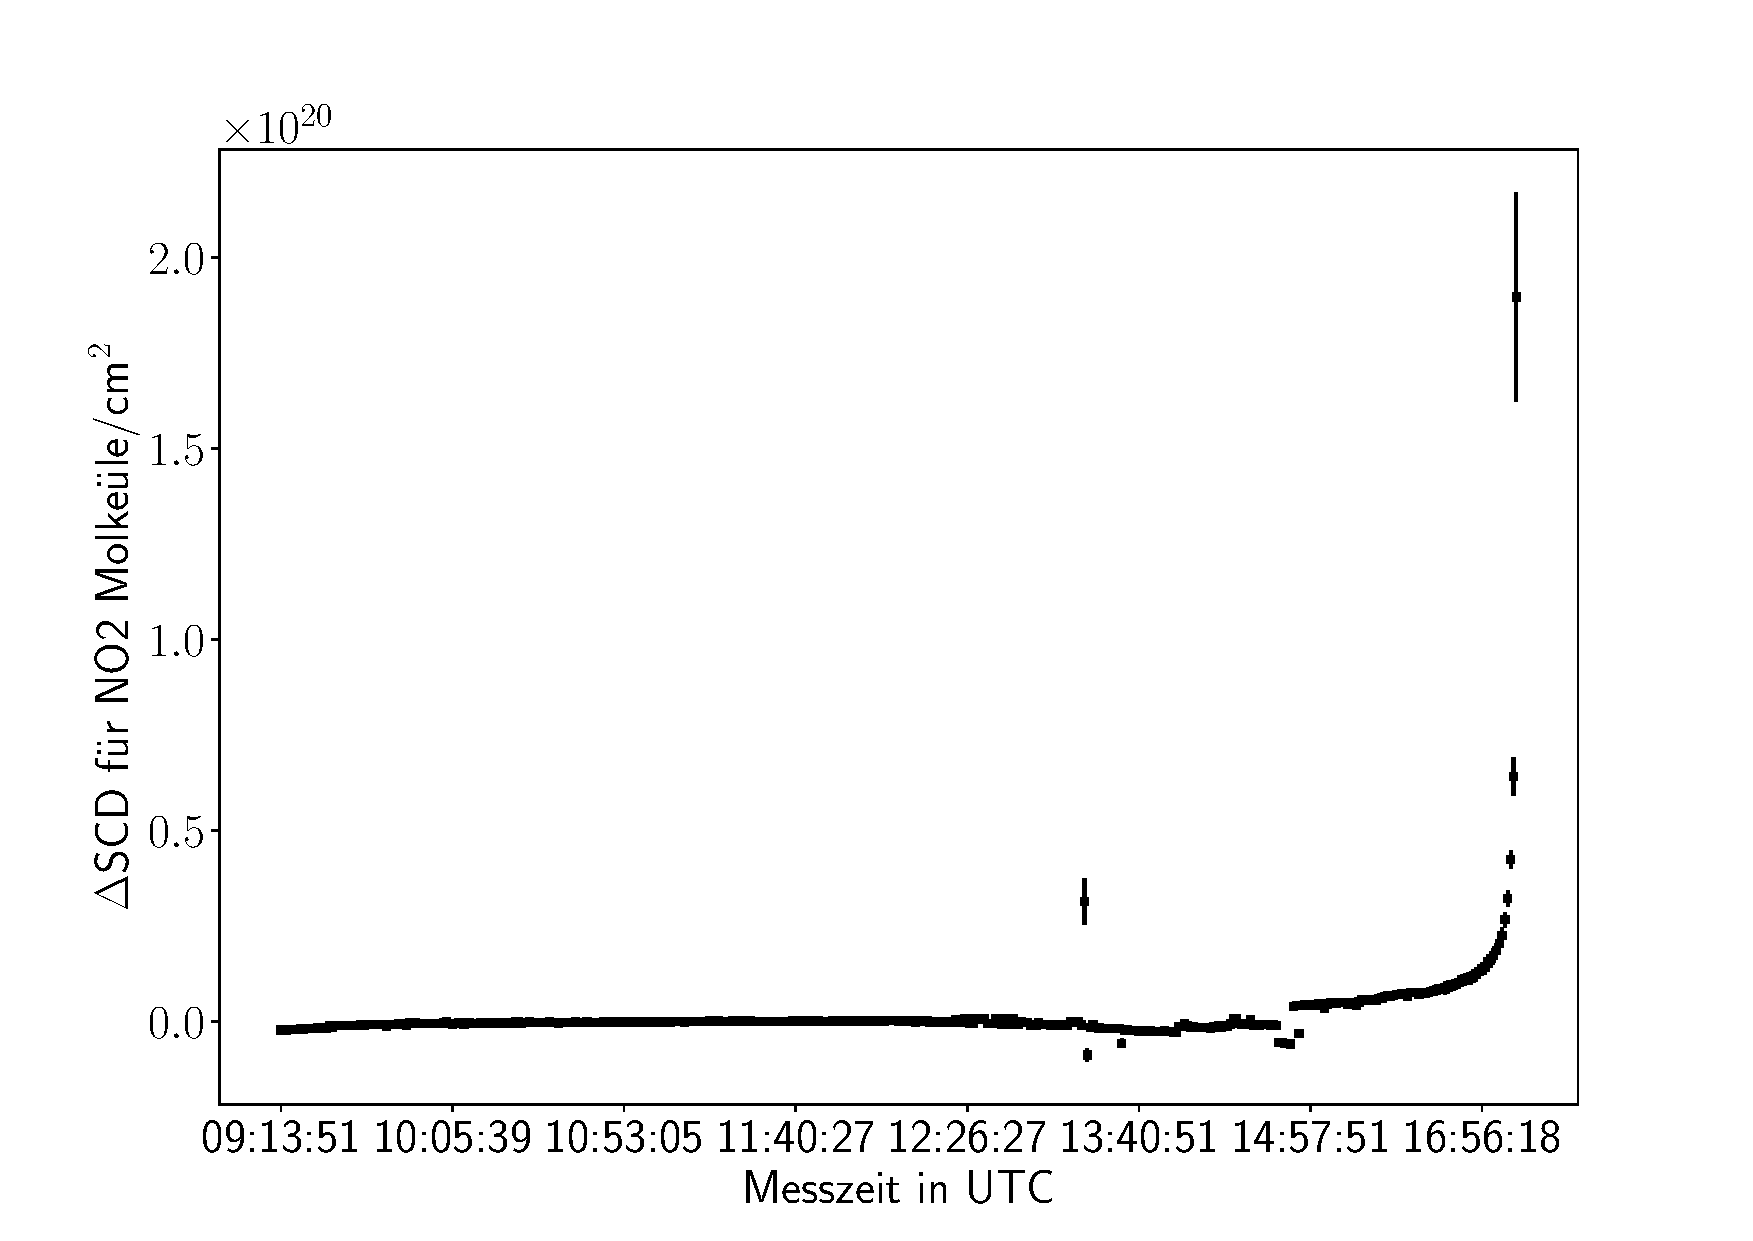
\includegraphics[width=.9\linewidth]{fig/SCD_Time_Plot_O3.pdf}
    \captionof{figure}{$\Delta \text{SCD}$ von \ch{O3} über den Tag des 24.04.    2019}
    \label{fig:delta_SCD_time_O3}
\end{center}
\end{frame}

\begin{frame}
    \frametitle{Tagesmessung \ch{O3}}
    \ch{O3} und \ch{NO2} sind im Gleichgewicht:
    \begin{align}
         \ch{O3} + \ch{NO} \rightleftharpoons \ch{NO2} + \ch{O2}
    \end{align}
    \ch{O3} Hauptsächlich in Stratosphäre
\end{frame}

\begin{frame}
    \frametitle{Langley Plots}
    $\Delta$ SCD wird gegen Air Mass Factor (AMF) aufgetragen\\
    \begin{align}
        \text{AMF}(\theta) := \frac{\text{SCD}(\theta)}{\text{VCD}} \approx \frac{1}{\cos (\theta)}
    \end{align}
    \begin{figure}
        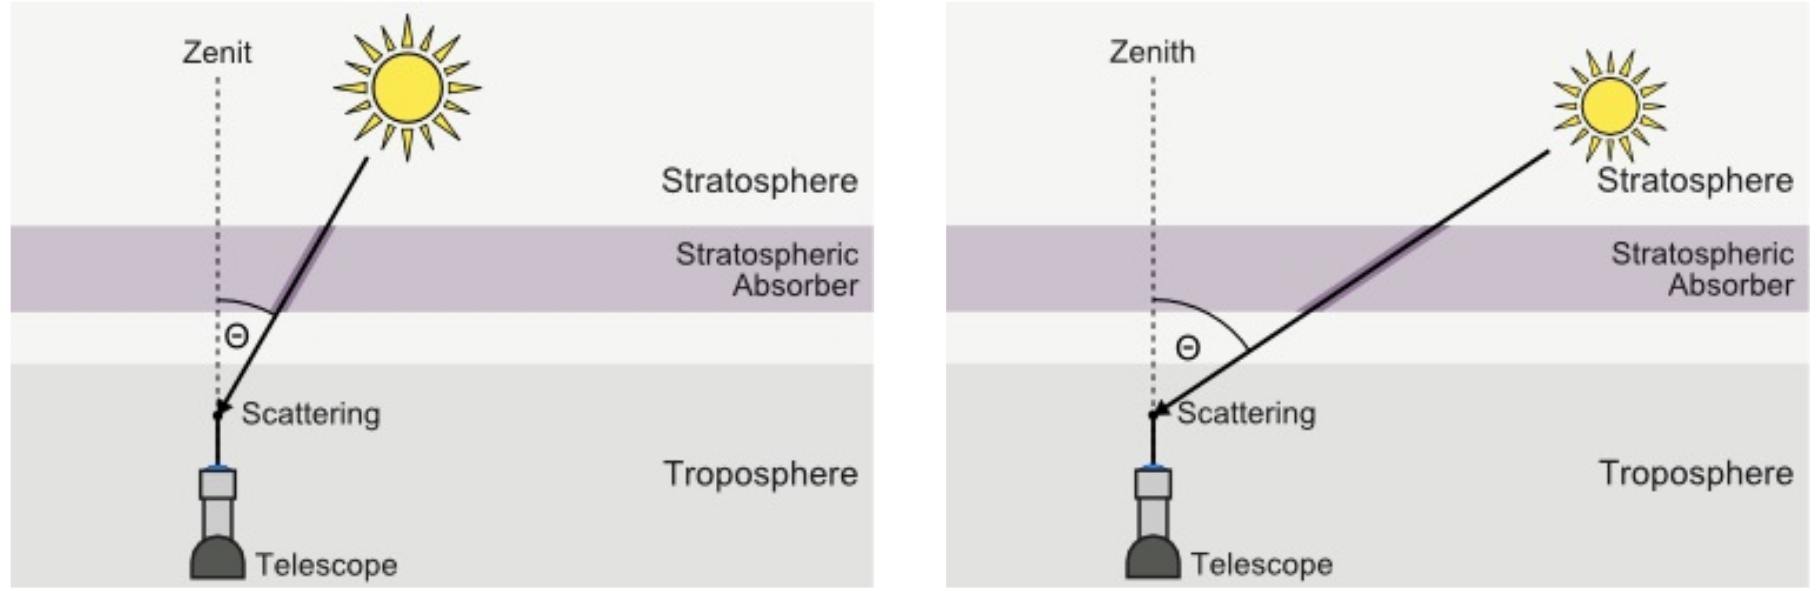
\includegraphics[width=0.9\linewidth]{fig/langley_sza.png}
    \end{figure}
\end{frame}

\begin{frame}
    \frametitle{Langley Plots}
    Die totale SCD ist $S = \Delta S + S_F$\\
    $S_F$ kann mit Langley Plot bestimmt werden\\
    Wenn Konzentration konstant $\to$ Linearer Langley Plot
    \begin{align}
    \Delta \text{SCD} = \text{VCD} A - S_F
    \end{align}
\end{frame}

\begin{frame}
    \frametitle{Langley Plot von \ch{NO2}}
    \begin{figure}
    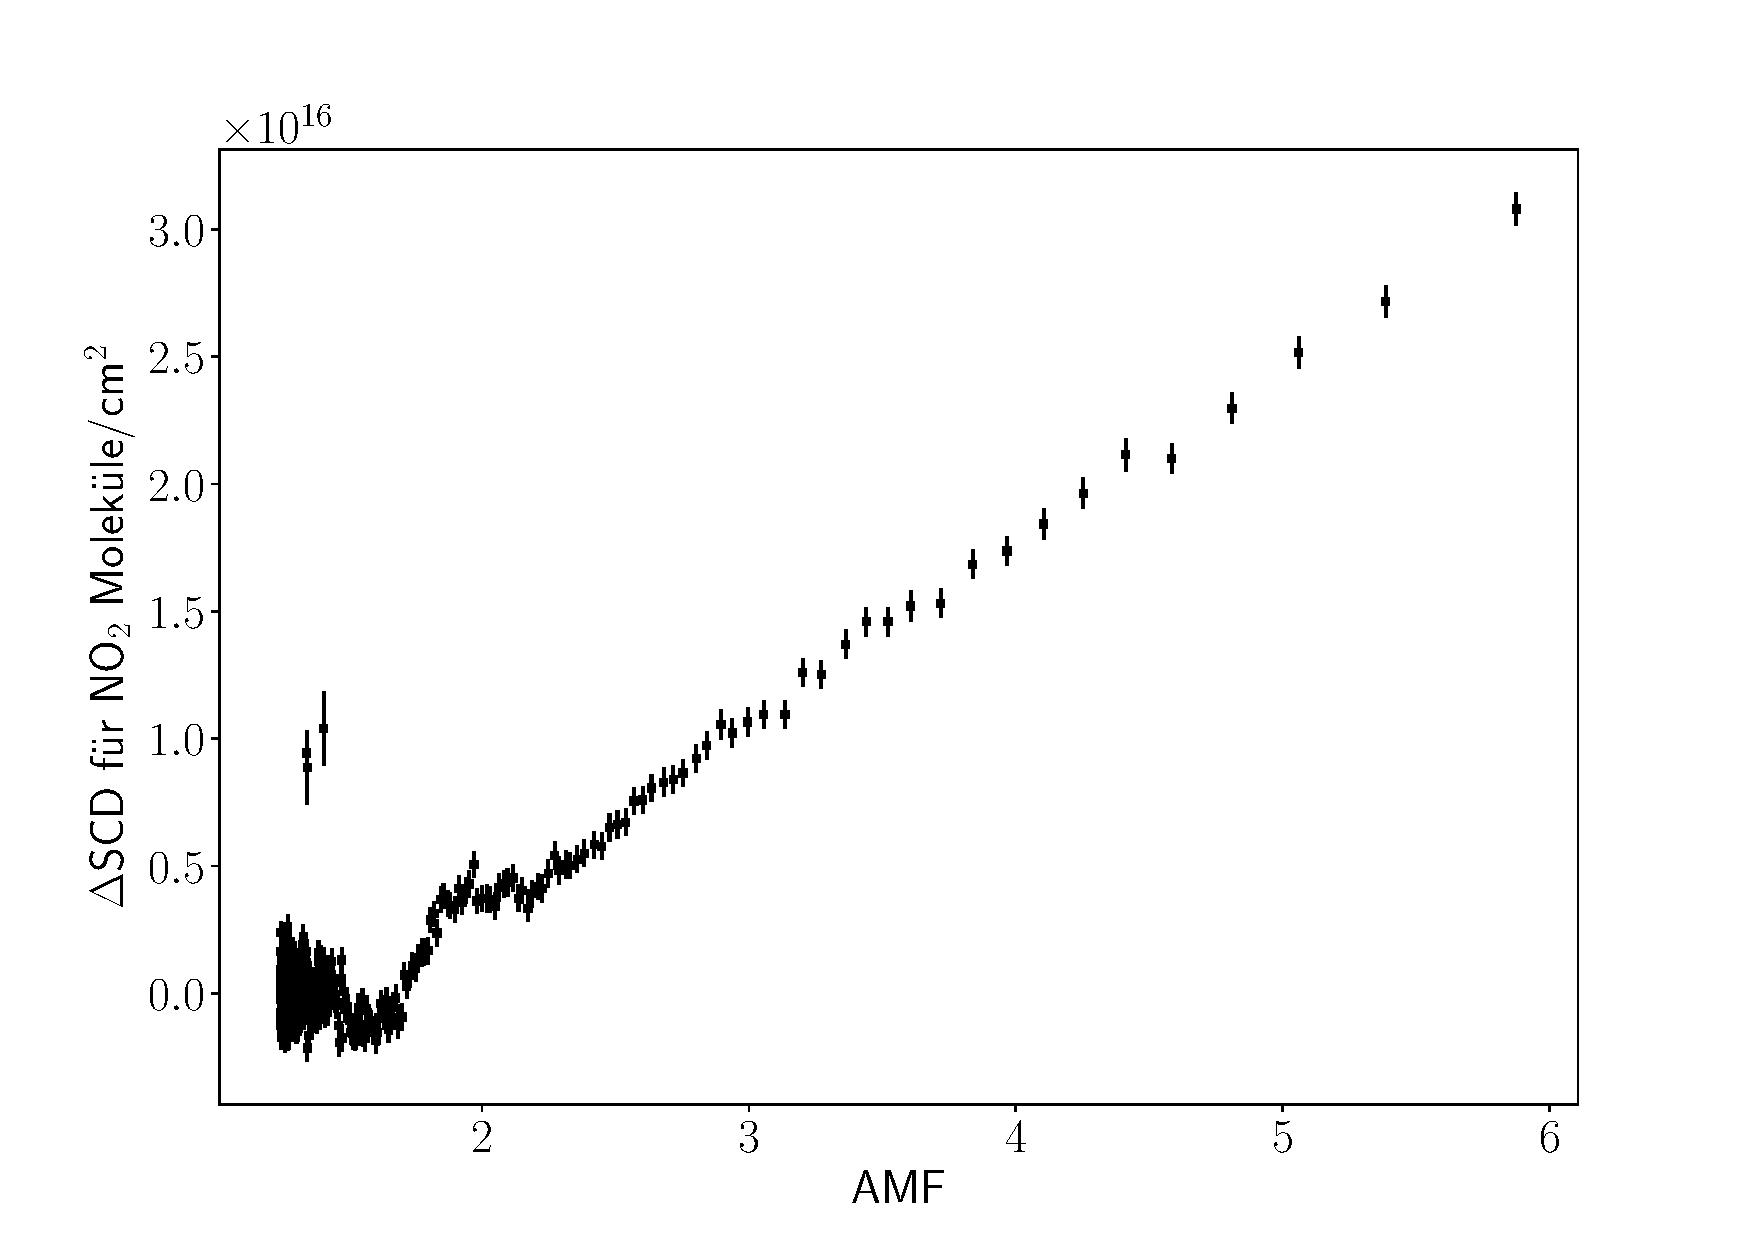
\includegraphics[width=.9\linewidth]{fig/Langley_Plot_NO2_cut.pdf}
    \end{figure}
\end{frame}

\begin{frame}
    \frametitle{Langley Plot von \ch{O3}}
    \begin{figure}
    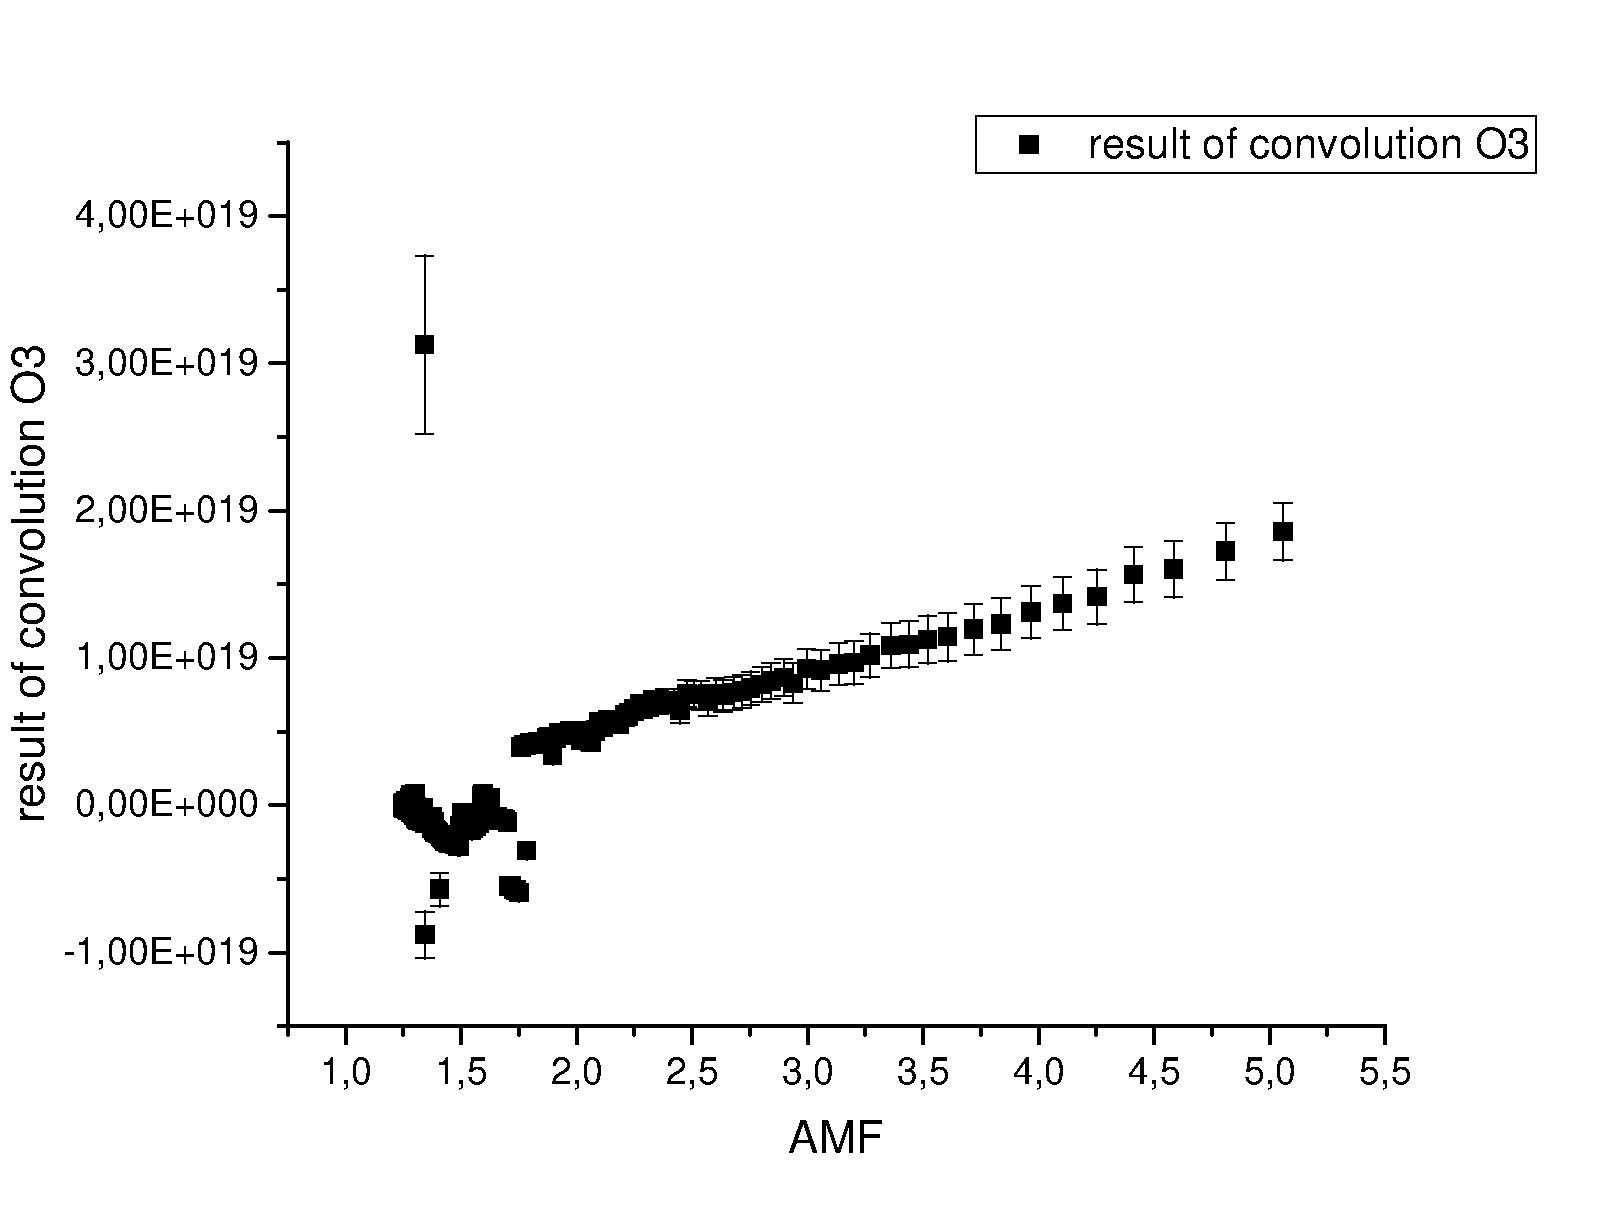
\includegraphics[width=.9\linewidth]{fig/Langley_Plot_O3_cut.pdf}
    \end{figure}
\end{frame}

\begin{frame}
    \frametitle{Fit $\Delta$SCD von \ch{O3}}
    \begin{figure}
    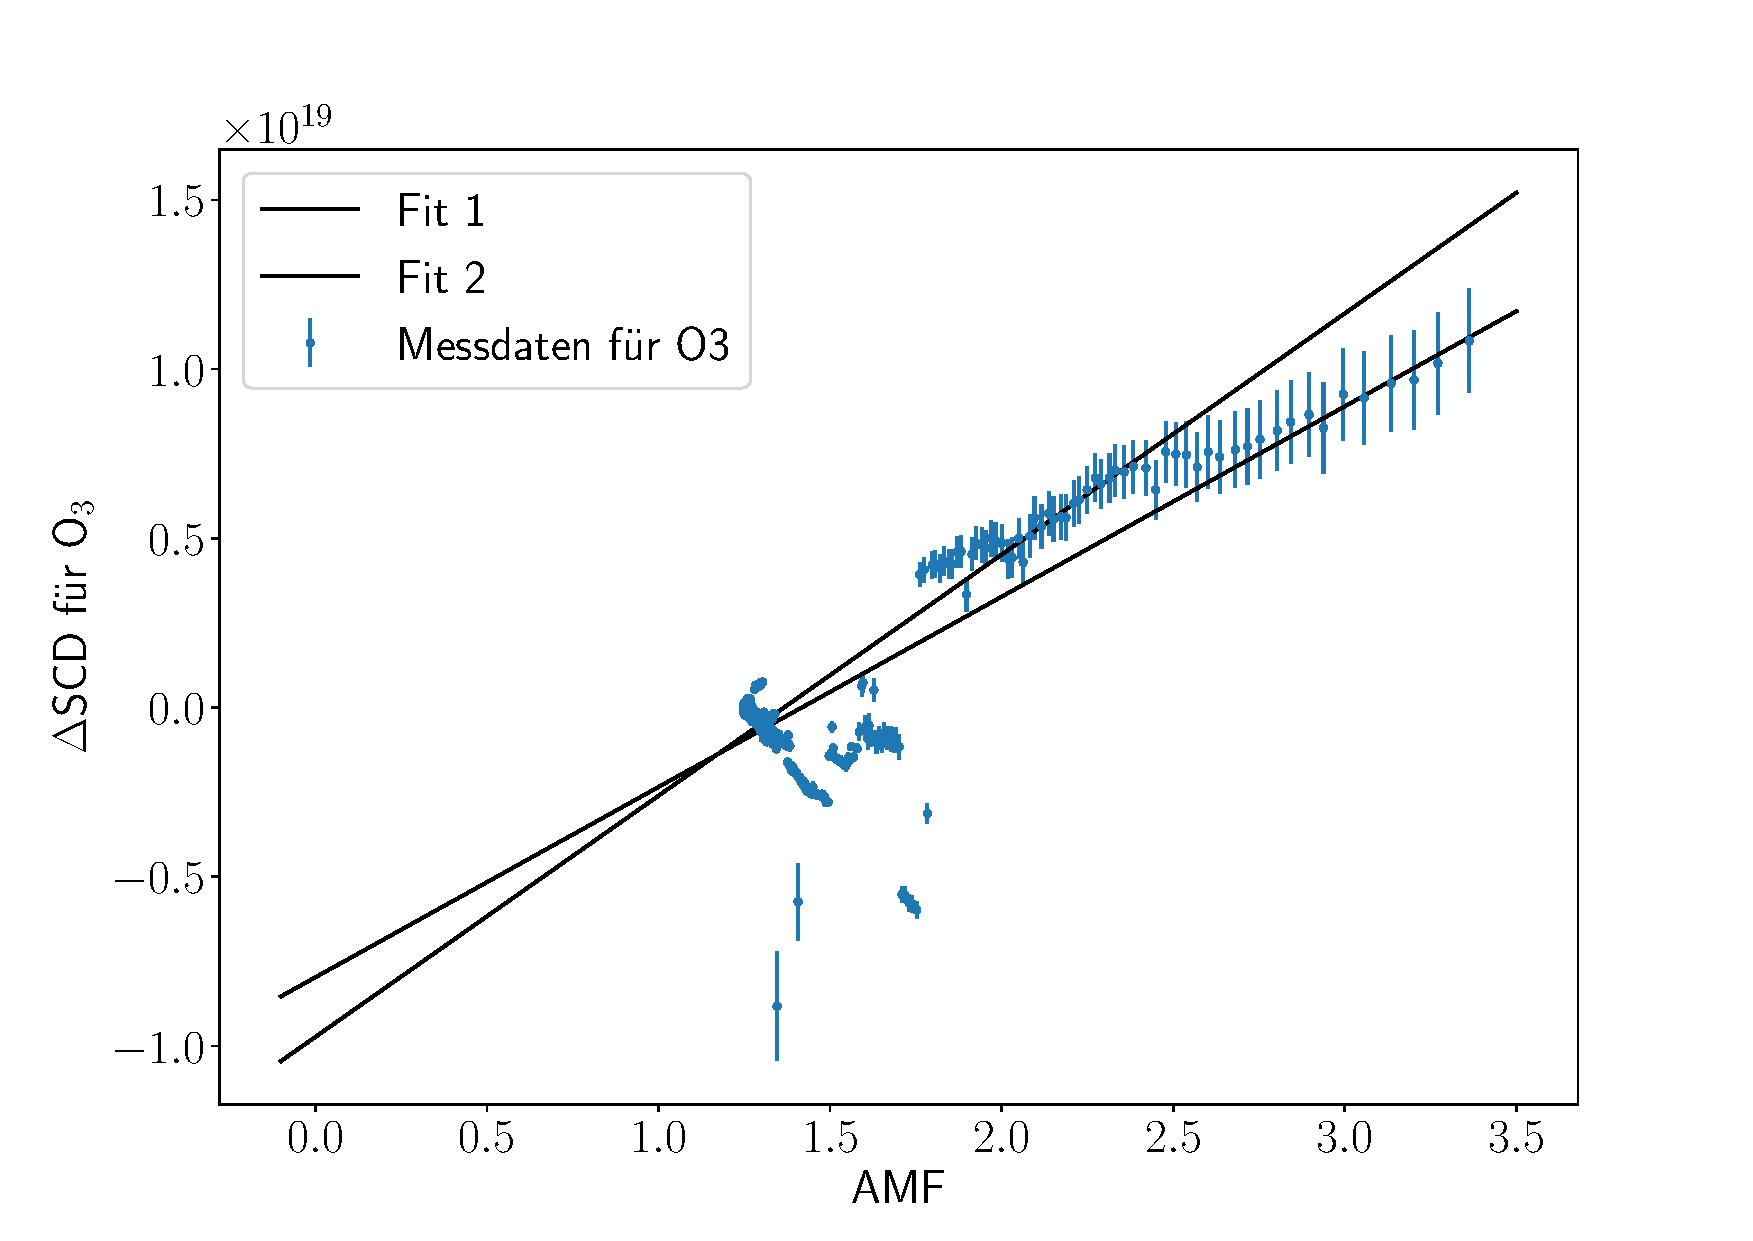
\includegraphics[width=.9\linewidth]{fig/scd_fit_o3.pdf}
    \end{figure}
\end{frame}

\begin{frame}
    \frametitle{Vertical Column Density \ch{O3}}
    Vertical Column Density (VCA) ist:
    \begin{align}
        \text{VCD} = \text{SCD} \cos (\theta)
    \end{align}
\end{frame} 

\begin{frame}
    \frametitle{Vertical Column Density \ch{O3}}
    \begin{figure}
    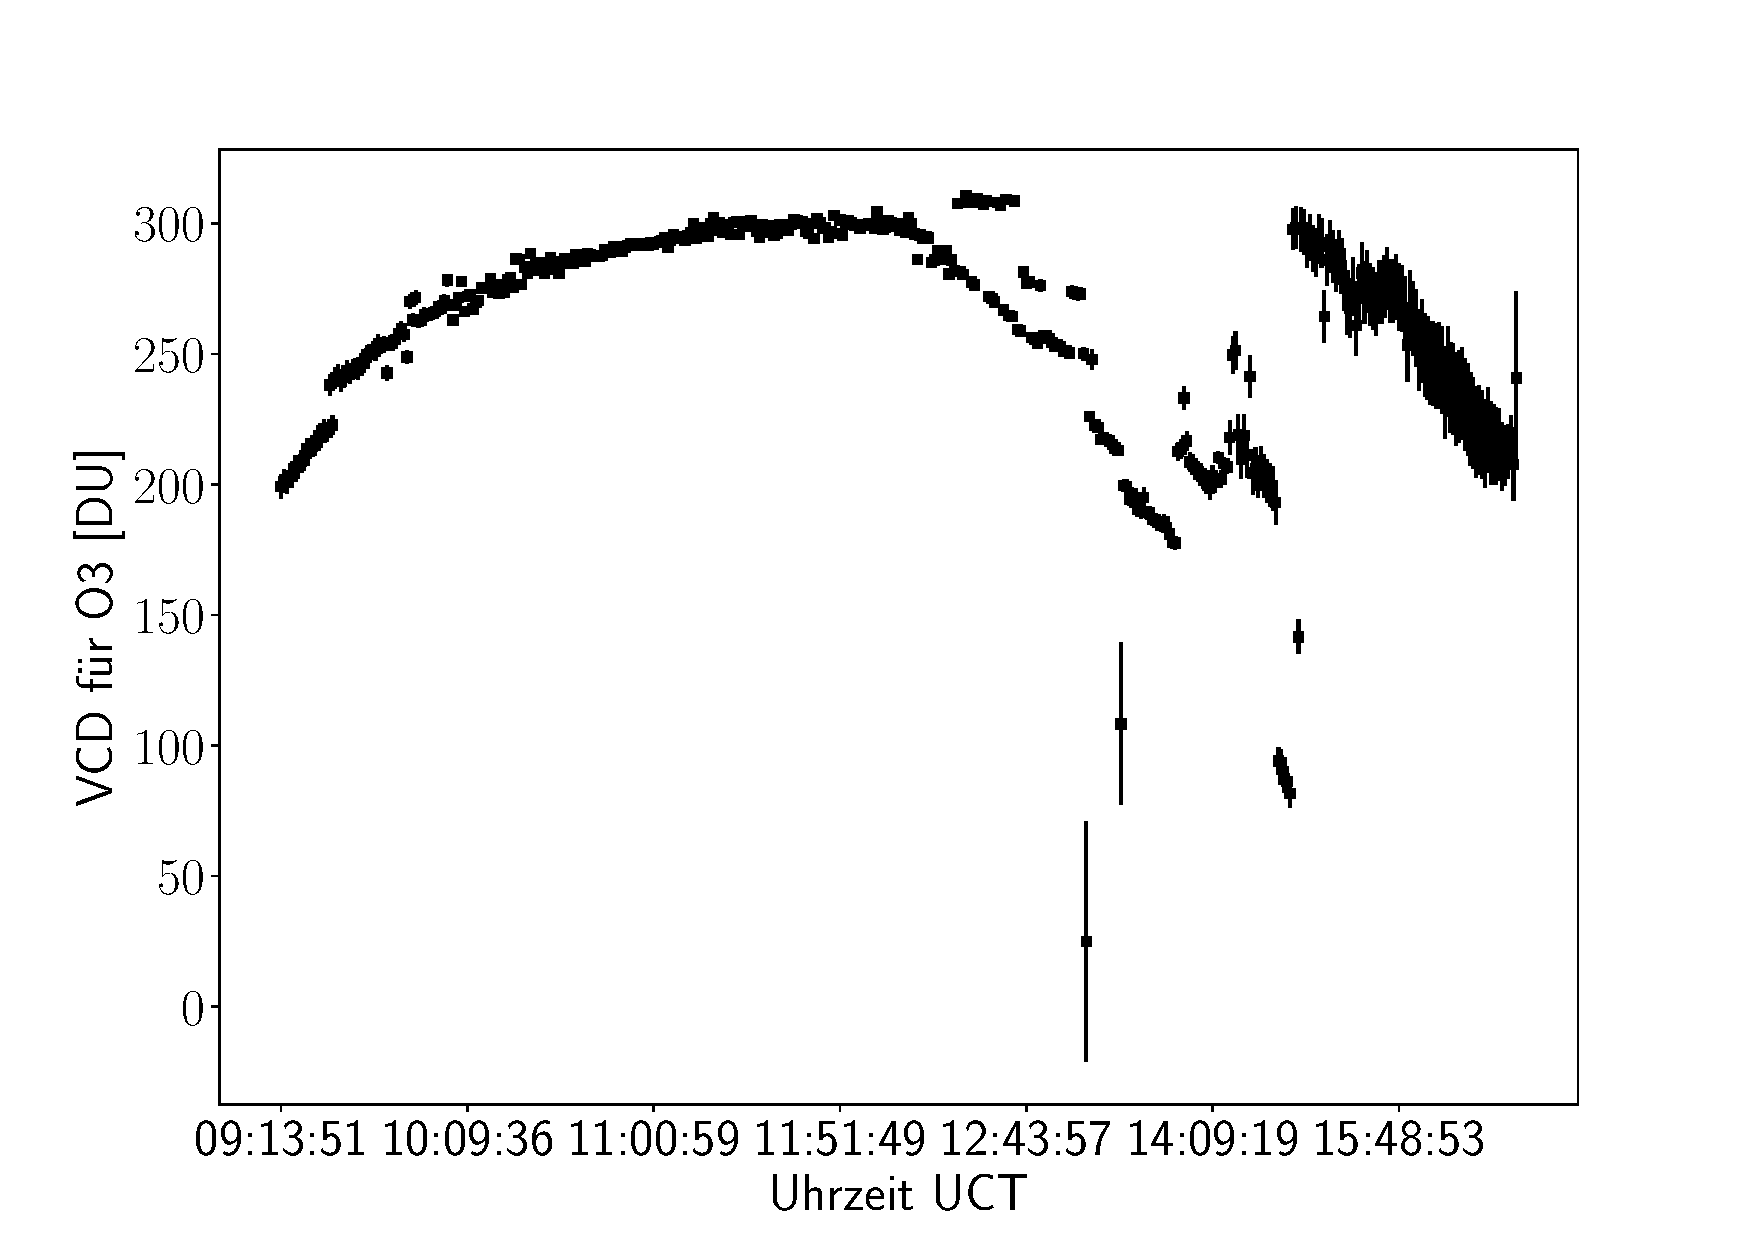
\includegraphics[width=.9\linewidth]{fig/VCD_O3_over_day.pdf}
    \end{figure}
\end{frame}

\begin{frame}
    \begin{figure}
    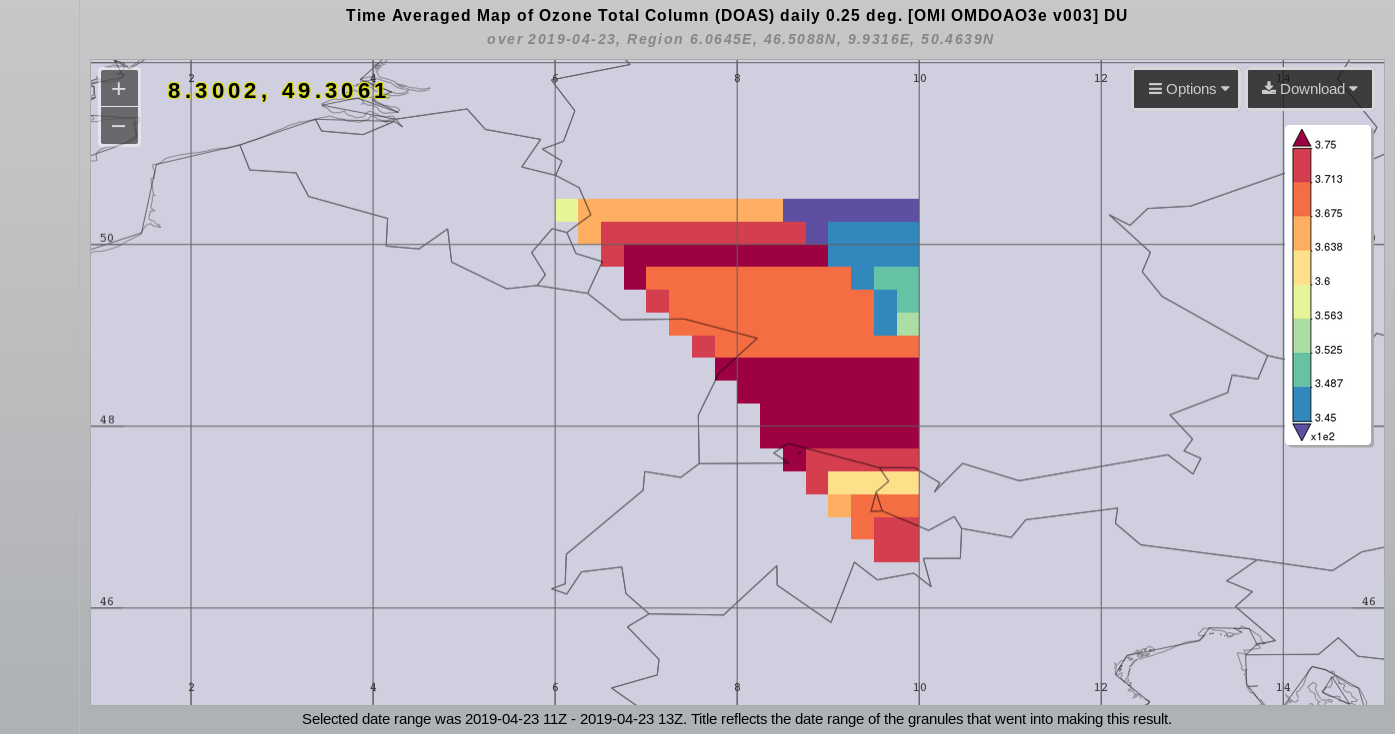
\includegraphics[width=.9\linewidth]{fig/DOAS_VCD_Ozone_ohne_Maus.png}
    \end{figure}

    \begin{figure}
    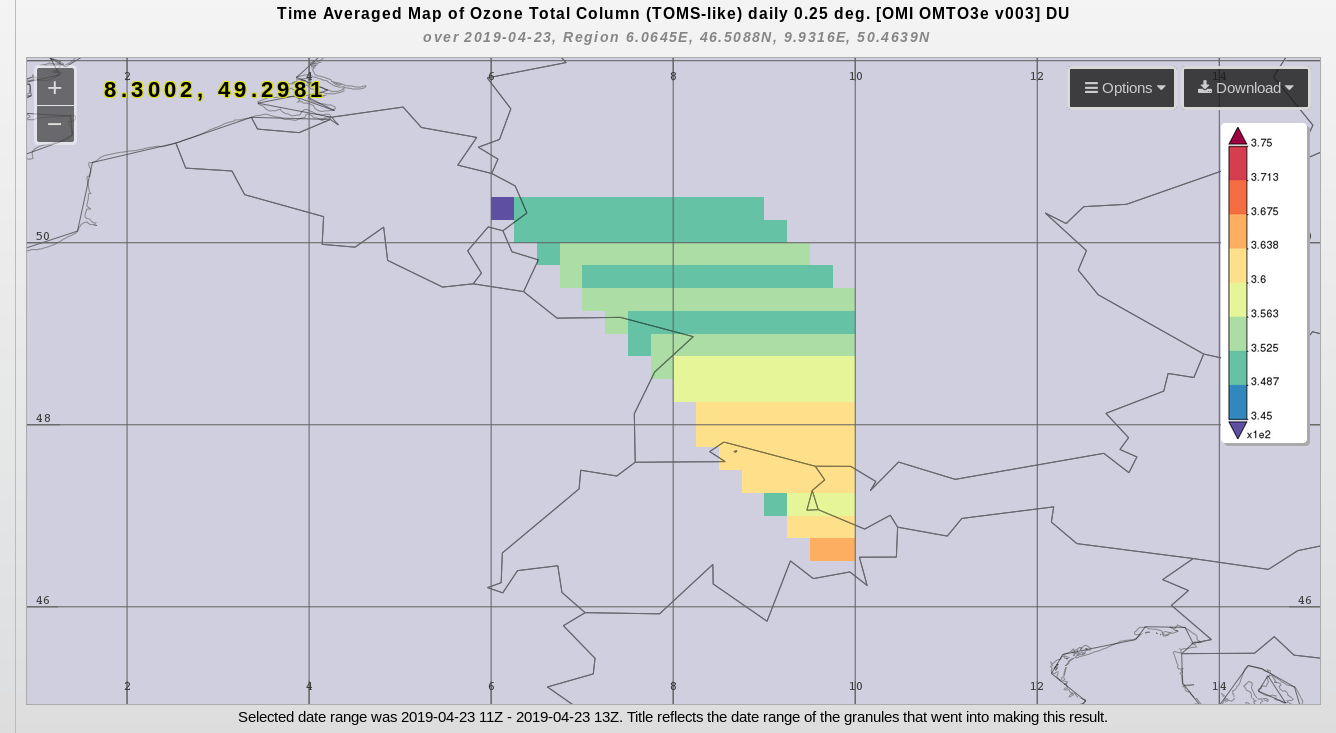
\includegraphics[width=.9\linewidth]{fig/TOMS_VCD_Ozone_ohne_Maus.png}
    \end{figure}
\end{frame}

\begin{frame}
    \frametitle{Multi Axis DOAS}
    Liefert Einblick in die vertikale Verteilung der Spurengase \\
    Jetzt $\alpha$: Winkel zwischen Horizont und Richtung der Kamera
    \begin{figure}
        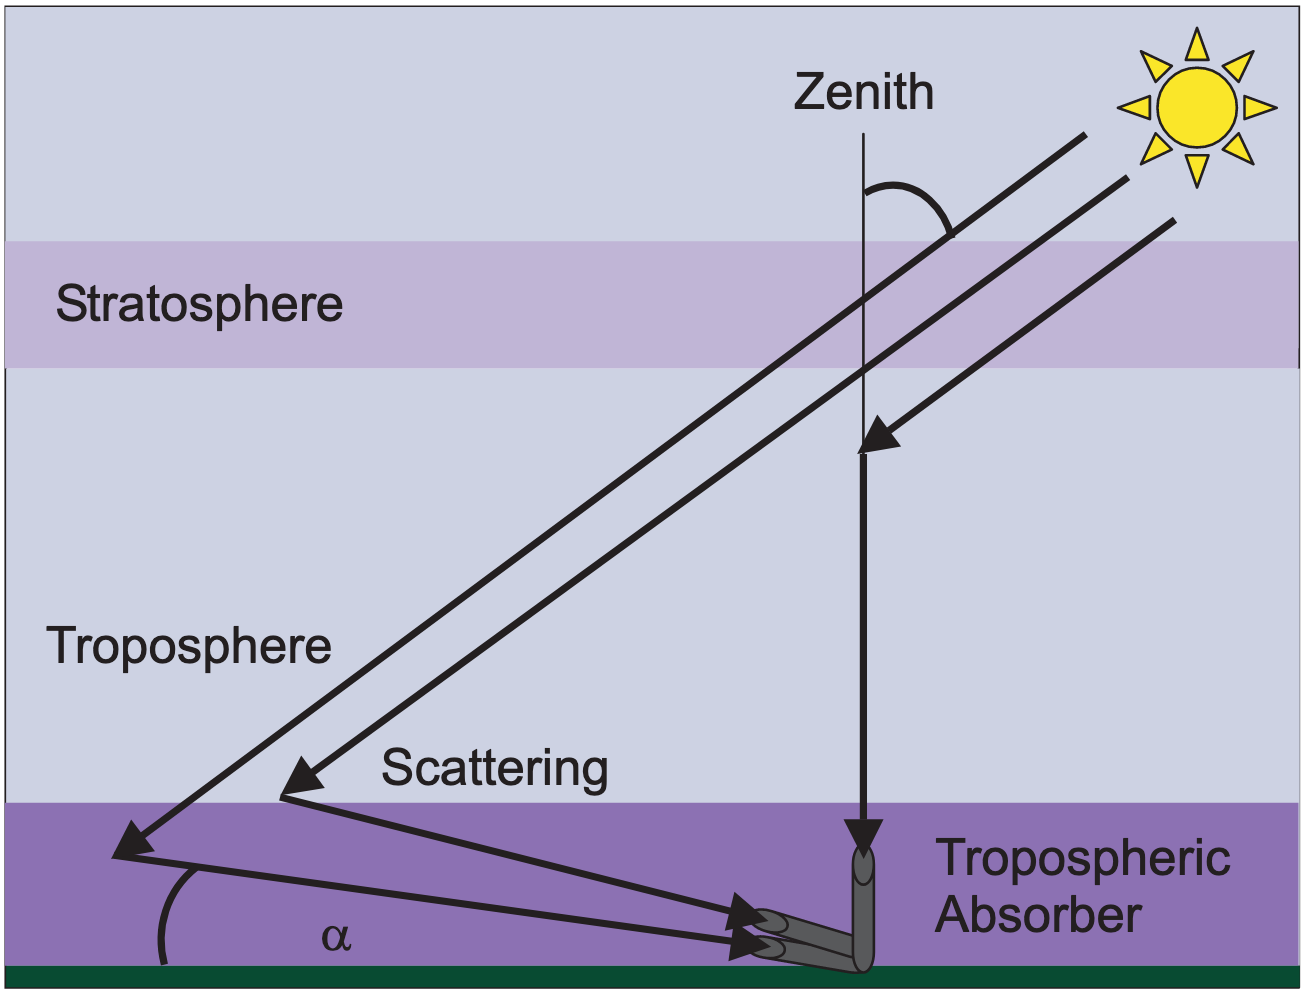
\includegraphics[width=.6\linewidth]{fig/photo/max_doas.png}
    \end{figure}
\end{frame}

\begin{frame}
    \frametitle{Multi Axis DOAS}
    Vier Messreihen bei jeweils $7^\circ$, $12^\circ$ und $90^\circ$ \\
    \begin{center}
    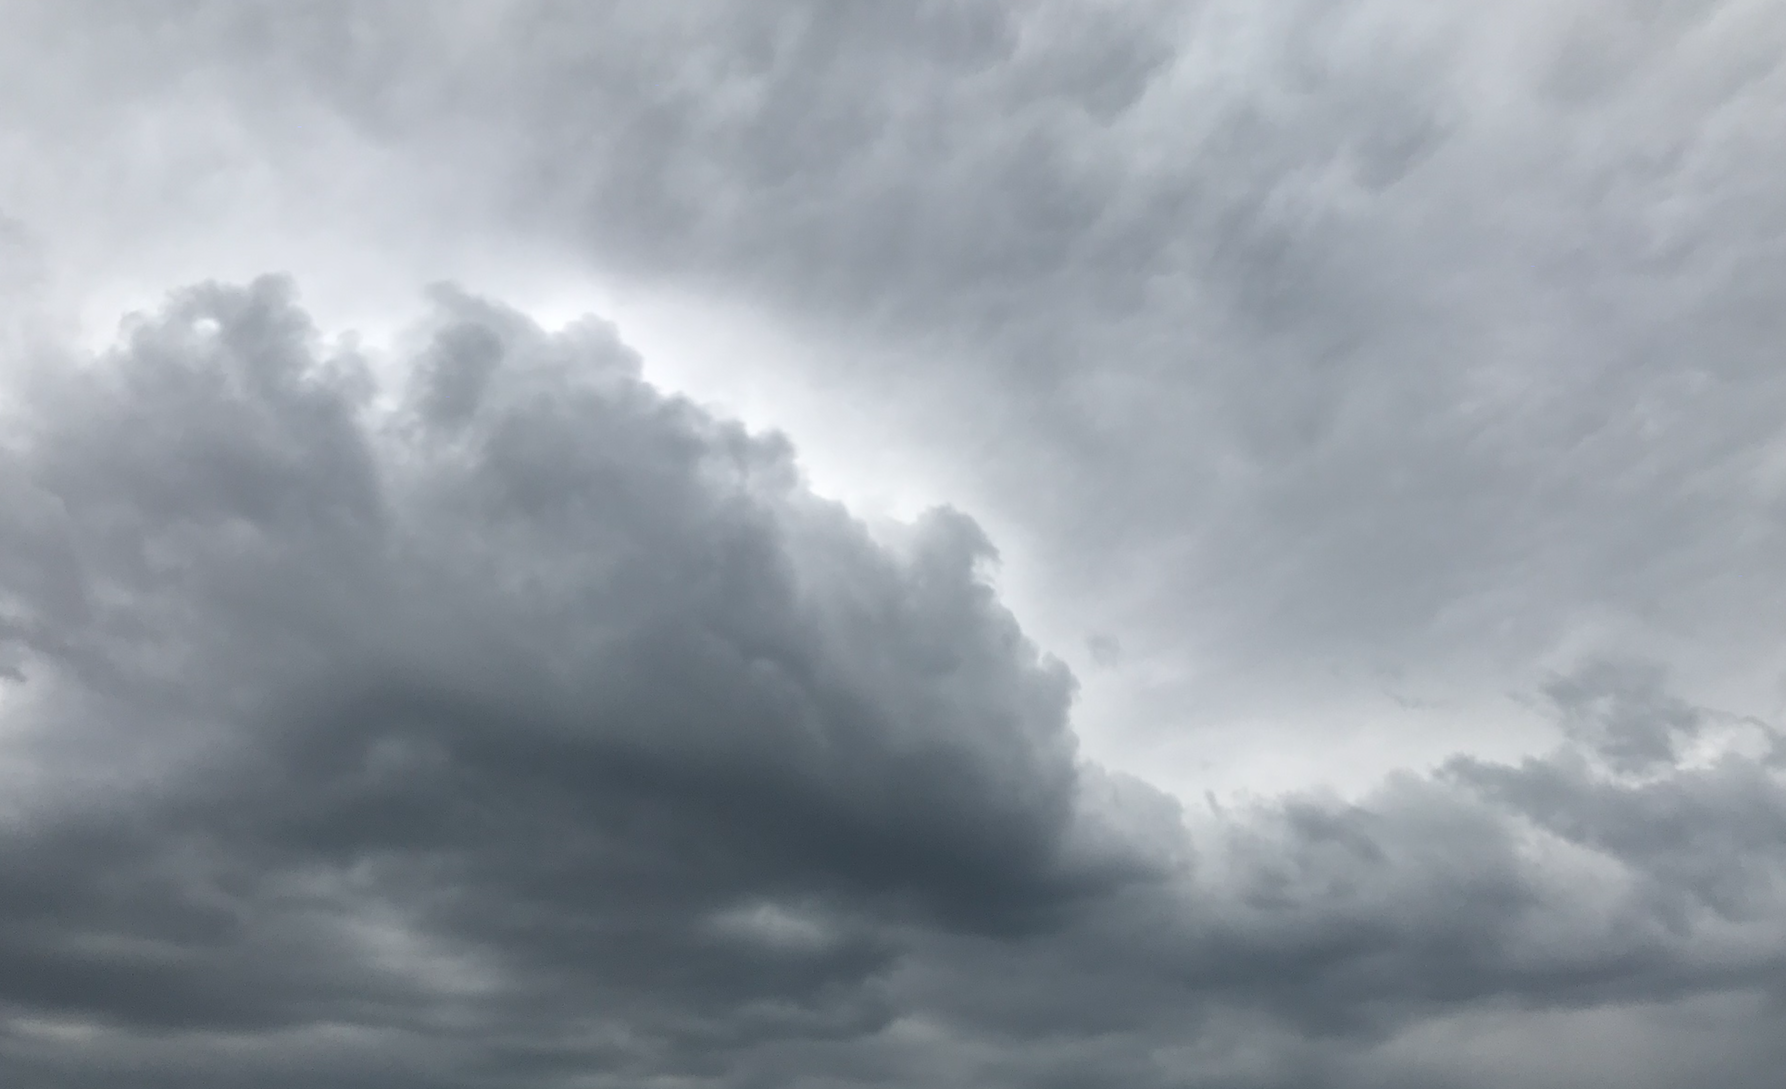
\includegraphics[width=.7\linewidth]{fig/photo/wetter.png}
    \end{center}
\end{frame}

\begin{frame}
    \frametitle{MAX-DOAS \ch{O3}}
    \begin{figure}
    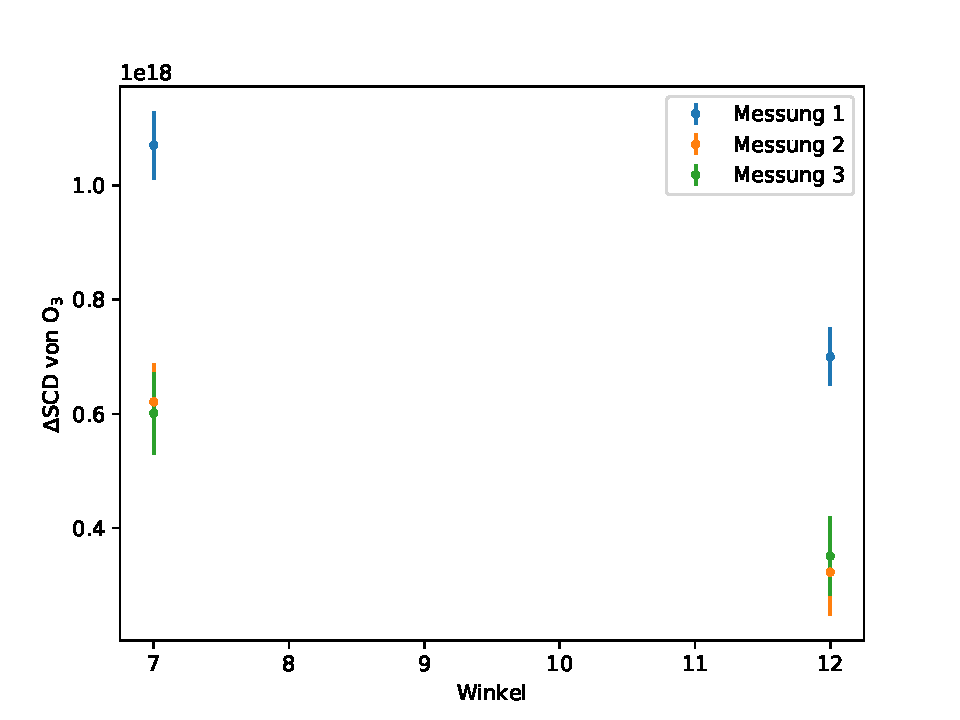
\includegraphics[width=0.9\linewidth]{fig/max_DOAS_O3.pdf}
    \end{figure}
\end{frame}

\begin{frame}
    \frametitle{MAX-DOAS \ch{NO2}}
    \begin{figure}
    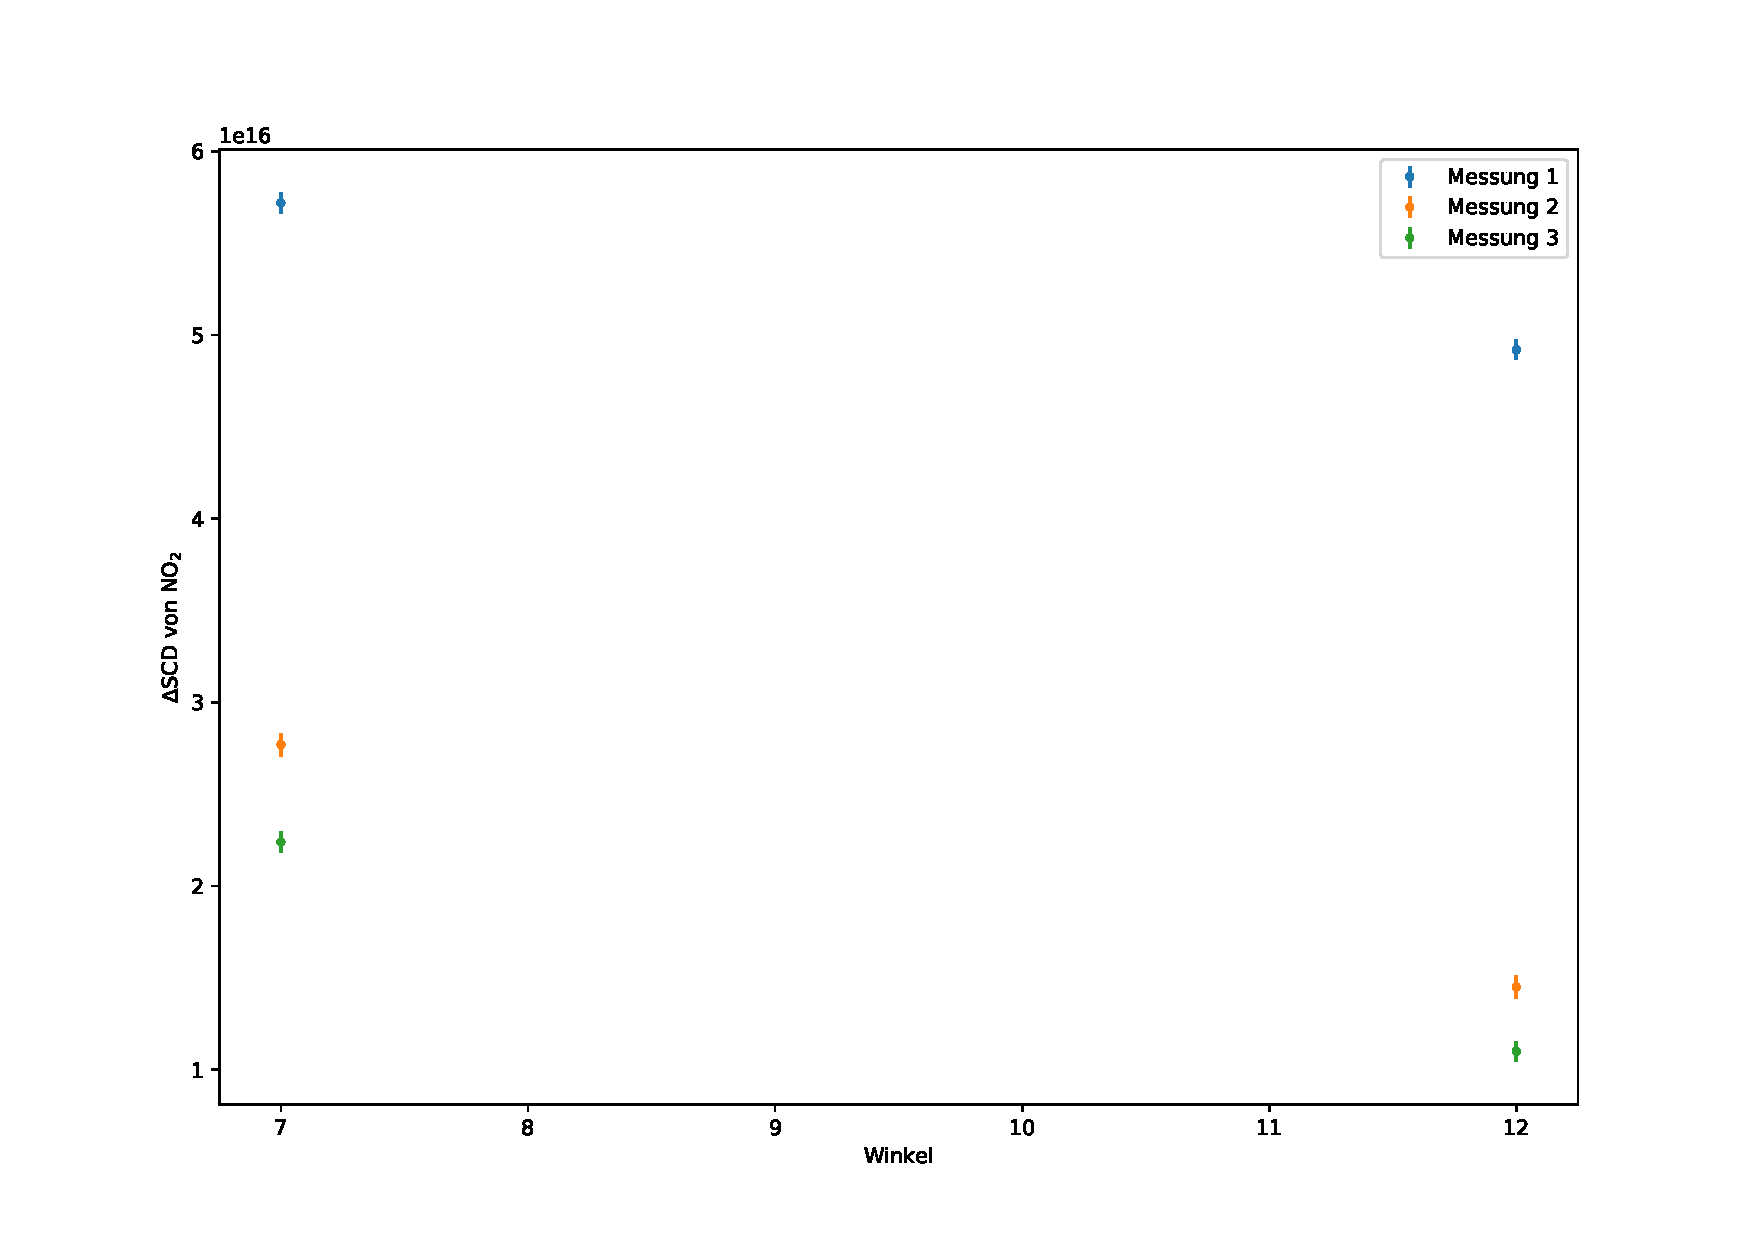
\includegraphics[width=0.9\linewidth]{fig/max_DOAS_NO2.pdf}
    \end{figure}
\end{frame}


\begin{frame}
    \frametitle{MAX-DOAS \ch{O4}}
    \begin{figure}
    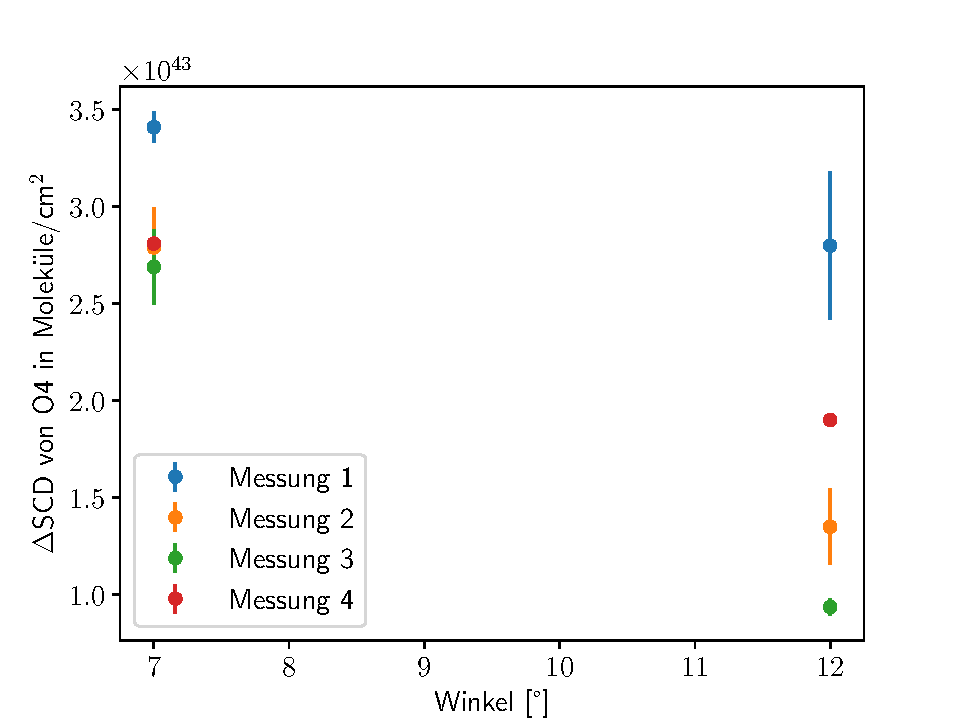
\includegraphics[width=0.9\linewidth]{fig/max_DOAS_O4.pdf}
    \end{figure}
\end{frame}


\begin{frame}
    \begin{center}
        \frametitle{MAX-DOAS Messung}
	\begin{tabular*}{\linewidth}{c c}
		\toprule
        Molekül & Verhältnis $\Delta \text{SCD}$ \\
        \midrule
        \ch{O3} & $1.0 \pm 0.4$ \\
        \ch{NO2} & $1.4 \pm 1.1$ \\
        \ch{O4} & $1.7 \pm 0.7$\\
		\bottomrule
	\end{tabular*}
    \captionof{table}{Verhältnis der $\Delta$SCD von \ch{O3}, \ch{NO2} und \ch{O4}}
	\label{fig:ratio_dscd}
\end{center}
\end{frame}
\end{document}
